\documentclass[xcolor=dvipsnames,12pt,aspectratio=169]{beamer}
\usecolortheme[named=violet]{structure} 

%\usetheme{umbc2} 
\usepackage{pgf}
%\usepackage[pdftex]{graphicx}
\usepackage{color}
\usepackage{amssymb,amsmath}
\usepackage[english]{babel}
\mode<presentation>

 \usepackage{multimedia}
\usefonttheme{structurebold}

%\useinnertheme{umbcboxes}

%\setbeamercolor{umbcboxes}{bg=violet!15,fg=black}  

\setbeamercovered{transparent}
\setbeamertemplate{navigation symbols}{}

%
%
% Adjustable parenthesis et al
%
\newcommand{\K}[1]{\left({#1}\right)}
\newcommand{\lp}{\left(}
\newcommand{\rp}{\right)}
\newcommand{\lb}{\left[}
\newcommand{\rb}{\right]}
\newcommand{\lc}{\left\{}
\newcommand{\rc}{\right\}}
\newcommand{\la}{\left\langle}
\newcommand{\ra}{\right\rangle}
\newcommand{\Dp}[3]{\langle #1,#2 \rangle_{#3}}
\newcommand{\cov}[2]{\langle #1\,#2 \rangle}

\newcommand{\half}{\mbox{$\frac{1}{2}$}} %

\newcommand{\U}{{\cal U}}
\newcommand{\C}{{\cal C}}
\newcommand{\X}{{\cal X}}
\newcommand{\Y}{{\cal Y}}

\newcommand {\ared} {{\rm ared}}
\newcommand {\pred} {{\rm pred}}
\newcommand {\rpred} {{\rm rpred}}

\newcommand{\sn}{s^{\sf n}}  % Normal component
\newcommand{\st}{s^{\sf t}}  % Tangential component
\newcommand{\rt}{r^{\sf t}}  % Tangential component
\newcommand{\stepy}{{s_y}}  % step in y--component
\newcommand{\stepu}{{s_u}}  % step in u--component

%
\newcommand{\veps}{{\varepsilon}} 
% Bolds and scripts
%
\newcommand{\CG}{\ensuremath{\mathcal{G}} }
\newcommand{\CQ}{\ensuremath{\mathcal{Q}} } %
\newcommand{\CR}{\ensuremath{\mathcal{R}} } %
\newcommand{\CW}{\ensuremath{\mathcal{W}} } %
\newcommand{\CX}{\ensuremath{\mathcal{X}} } %
\newcommand{\CZ}{\ensuremath{\mathcal{Z}} } %
\newcommand{\CU}{\ensuremath{\mathcal U} }
\newcommand{\CC}{\ensuremath{\mathcal C} }
\newcommand{\CD}{\ensuremath{\mathcal D} }
\newcommand{\BA}{\ensuremath{\mathbf{A}} } %
\newcommand{\BB}{\ensuremath{\mathbf{B}} } %
\newcommand{\BC}{\ensuremath{\mathbf{C}} } %
\newcommand{\BhC}{\ensuremath{\widehat{\mathbf{C}}} } %
\newcommand{\BD}{\ensuremath{\mathbf{D}} } %
\newcommand{\BE}{\ensuremath{\mathbf{E}} } %
\newcommand{\BF}{\ensuremath{\mathbf{F}} } %
\newcommand{\BG}{\ensuremath{\mathbf{G}} } %
\newcommand{\BH}{\ensuremath{\mathbf{H}} } %
\newcommand{\BK}{\ensuremath{\mathbf{K}} } %
\newcommand{\BL}{\ensuremath{\mathbf{L}} } %
\newcommand{\BM}{\ensuremath{\mathbf{M}} } %
\newcommand{\BN}{\ensuremath{\mathbf{N}} } %
\newcommand{\BP}{\ensuremath{\mathbf{P}} } %
\newcommand{\BQ}{\ensuremath{\mathbf{Q}} } %
\newcommand{\BR}{\ensuremath{\mathbf{R}} } %
\newcommand{\BU}{\ensuremath{\mathbf{U}} } %
\newcommand{\BW}{\ensuremath{\mathbf{W}} } %
\newcommand{\BX}{\ensuremath{\mathbf{X}} } %
\newcommand{\BY}{\ensuremath{\mathbf{Y}} } %
\newcommand{\BZ}{\ensuremath{\mathbf{Z}} } %
\newcommand{\ba}{\ensuremath{\mathbf{a}}}
\newcommand{\bb}{\ensuremath{\mathbf{b}}}
\newcommand{\bc}{\ensuremath{\mathbf{c}}}
\newcommand{\be}{\ensuremath{\mathbf{e}}}
\newcommand{\bg}{\ensuremath{\mathbf{g}}} %
\newcommand{\bh}{\ensuremath{\mathbf{h}}} %
\newcommand{\bk}{\ensuremath{\mathbf{k}}} %
\newcommand{\bn}{\ensuremath{\mathbf{n}}} %
\newcommand{\bp}{\ensuremath{\mathbf{p}}} %
\newcommand{\bq}{\ensuremath{\mathbf{q}}}
\newcommand{\br}{\ensuremath{\mathbf{r}}} %
\newcommand{\bs}{\ensuremath{\mathbf{s}}} %
\newcommand{\bt}{\ensuremath{\mathbf{t}}} %
\newcommand{\bu}{\ensuremath{\mathbf{u}}} %
\newcommand{\bv}{\ensuremath{\mathbf{v}}} %
\newcommand{\bdv}{\ensuremath{\mathbf{\delta v}}} %
\newcommand{\bw}{\ensuremath{\mathbf{w}}} %
\newcommand{\bd}{\ensuremath{\mathbf{d}}} %
\newcommand{\bx}{\ensuremath{\mathbf{x}}} %
\newcommand{\by}{\ensuremath{\mathbf{y}}} %
\newcommand{\obx}{\ensuremath{\overline{\mathbf{x}}}} %
\newcommand{\oby}{\ensuremath{\overline{\mathbf{y}}}} %
\newcommand{\obz}{\ensuremath{\overline{\mathbf{z}}}} %
\newcommand{\obw}{\ensuremath{\overline{\mathbf{w}}}} %
\newcommand{\bz}{\ensuremath{\mathbf{z}}} %
\newcommand{\blambda}{\mbox{\boldmath $\lambda$}}
\newcommand{\bdelta}{\mbox{\boldmath $\delta$}}
\newcommand{\bxi}{\mbox{\boldmath{$\xi$}}}
\newcommand{\bfeta}{\mbox{\boldmath $\eta$}}
\newcommand{\bkappa}{\mbox{\boldmath $\kappa$}}
\newcommand{\bmu}{\mbox{\boldmath $\mu$}}
\newcommand{\brho}{\mbox{\boldmath $\rho$}}
\newcommand{\bsigma}{\mbox{\boldmath $\sigma$}}
\newcommand{\sbxi}{\mbox{\scriptsize \boldmath{$\xi$}}}
\newcommand{\sbfeta}{\mbox{\scriptsize \boldmath $\eta$}}
\newcommand{\teta}{\mbox{\tiny \boldmath $\eta$}}
\newcommand{\txi}{\mbox{\tiny \boldmath{$\xi$}}}
\newcommand{\bLambda}{\mbox{\boldmath $\Lambda$}}
\newcommand{\bDelta}{\mbox{\boldmath $\Delta$}}
\newcommand{\bzero}{\mbox{\boldmath $0$}}
\newcommand{\bone}{\mbox{\boldmath $1$}}
\newcommand{\sDelta}{\mbox{\small $\Delta$}}
\newcommand{\tDelta}{\mbox{\tiny $\Delta$}}

\newcommand{\pd}[2]{\frac{\partial #1}{\partial #2}}
\newcommand{\ppd}[3]{\frac{\partial^{#3} #1}{\partial {#2}^{#3}}}
\newcommand{\pdsec}[3]{\frac{\partial^2 #1}{\partial #2\partial #3}}

\def\frechet{Fr\'echet\ }
%\newcommand{\real}{\mathbb{R}}
\newcommand{\real} {I\!\!R}
\newcommand{\nat} {{I\!\!N}}
\newcommand{\compl} {C\!\!\!\!I\;}
%
\def\Pr{\sf Pr}
\def\Re{\sf Re}
\def\M{{\sf M}}
\def\d{\delta}
\newcommand{\deq}{\raisebox{0pt}[1ex][0pt]{$\stackrel{\scriptscriptstyle{\rm def}}{{}={}}$}}
\newcommand{\dif}{{\mathrm d}}

\newcommand{\eref}[1]{\mbox{\rm(\ref{#1})}}
\newcommand{\tref}[1]{\mbox{\rm\ref{#1}}}


%\newenvironment{proof}{\noindent {\bf Proof:} }{\hfill $\Box$ \\[2ex] }

\newcommand{\myint}[1]{\int_0^T \dif t~{#1}}
\newcommand{\myintt}[1]{\int_0^1 \dif s~{#1}}
\newcommand{\dint}[1]{\int\limits_{#1}\!\!\!\int}

\newcommand{\waveop}[1]{c^{-2}{#1}_{tt}-\Delta{#1}}
\newcommand{\redwaveop}[1]{\Delta{#1}+k^2n^2{#1}}

\newcommand{\D}{\displaystyle}
%\allowdisplaybreaks
%

\setlength{\parskip}{2ex}   % place a blank line between paragraphs
\def\Logo{\@ifnextchar(\beamer@Logo\logo}
\def\beamer@Logo(#1,#2){\logo}

\AtBeginSection[]{
{\setbeamertemplate{logo}{}
 \begin{frame}<beamer>
    \frametitle{Agenda}
    \tableofcontents[currentsection]
  \end{frame}
}
}
% Images
% Macros
\newcommand{\peq}{\,+\hspace{-0.15cm}=}
\newcommand{\bm}{\bar{m}}
\newcommand{\dm}{\delta m}
\newcommand{\dom}{\delta \bar{m}}
\newcommand{\doma}{\delta \bar{m}_{\alpha}}
\newcommand{\om}{\bar{m}}
\newcommand{\bH}{{\bf H}}
\newcommand{\bR}{{\bf R}}
\newcommand{\bcF}{{\bar{\cal F}}}
\newcommand{\cF}{{\cal F}}
\newcommand{\oF}{\bar{F}}
\newcommand{\of}{\bar{f}}
\newcommand{\ou}{\bar{u}}
\newcommand{\odF}{\bar{F}^{\dagger}}
\newcommand{\oS}{\bar{S}}
\newcommand{\oM}{\bar{M}}
\newcommand{\oJa}{\bar{J}_{\alpha}}
\newcommand{\Na}{N_{\alpha}}
\newcommand{\dd}{\delta d}
\newcommand{\ddl}{\delta d_{\alpha}}
\title[]{Waveform Inversion via Source Extension}
\author[]{William W. Symes \inst{1}}
\institute[]{\inst{1} Rice University}
\date{Workshop in honor of Jean Virieux \\June 2025}

\begin{document}
\frame{
\titlepage
}

\renewcommand{\thefootnote}{\fnsymbol{footnote}}

%\begin{frame}\frametitle{The Plan}
%\begin{itemize}
%\item What is ``extended modeling", and why bother
%\item FWI via surface source extension - examples
%\item Theory: why \& when it works
%\item Zoology of source extensions
%\end{itemize}
%\end{frame}

\section{Inversion}

\begin{frame}%\frametitle{Conventional FWI}
FWI: adjust model parameters to make predicted data close to
observed data.

Predicted data = $Ru$, $u$ = modeled wavefield in space-time, $R$ =
sampling operator. Depends on $m$ = model parameters through wave equation
\[
L[m]u = s 
\]
$L[m]$ = wave operator, $s$ = energy source wavefield, Predicted data: $= F[m]s$, $F[m] = RL[m]^{-1}$ =
modeling operator

Least squares (``FWI''): given observed data $d$, source $s$, find $m$ to minimize
\[
J_{\rm FWI}[m] = \sum (F[m]s - d)^2
\]
$\sum$ = sum over all sources, receivers, times
\end{frame}

\begin{frame}
How to do it?

\begin{itemize}
\item Modeling (computing $u$ etc.): many methods - e.g. time-domain
  staggered grid finite differernce (\textcolor{blue}{Virieux}, 84)
\vspace{0,5cm}
\item Iterative descent update using gradient $\nabla J_{\rm FWI}$ - efficient
  computation via {\em adjoint state method} (Chavent-Lemmonier
  74,...), first multi-D demo by Gauthier-\textcolor{blue}{Virieux}-Tarantola 86
\end{itemize}

So what happens?
\end{frame}

\begin{frame}
A simple example: acoustic lens with isotropic point source @ $\bx_s$:
$f = w(t)\delta(\bx-\bx_s)$, $\bx_s$ = source position\\
%\[
%\frac{1}{\kappa}\frac{\partial p}{\partial t} = -\nabla \cdot {\bf v} + w(t)\delta(\bx-\bx_s), \,\rho \frac{\partial {\bf v}}{\partial t} = - \nabla p; \,p,{\bf v}=0, t \ll 0
%\]
%\vspace{-1.25in}
\vspace{-0.25in}
%\hspace{-0.5in}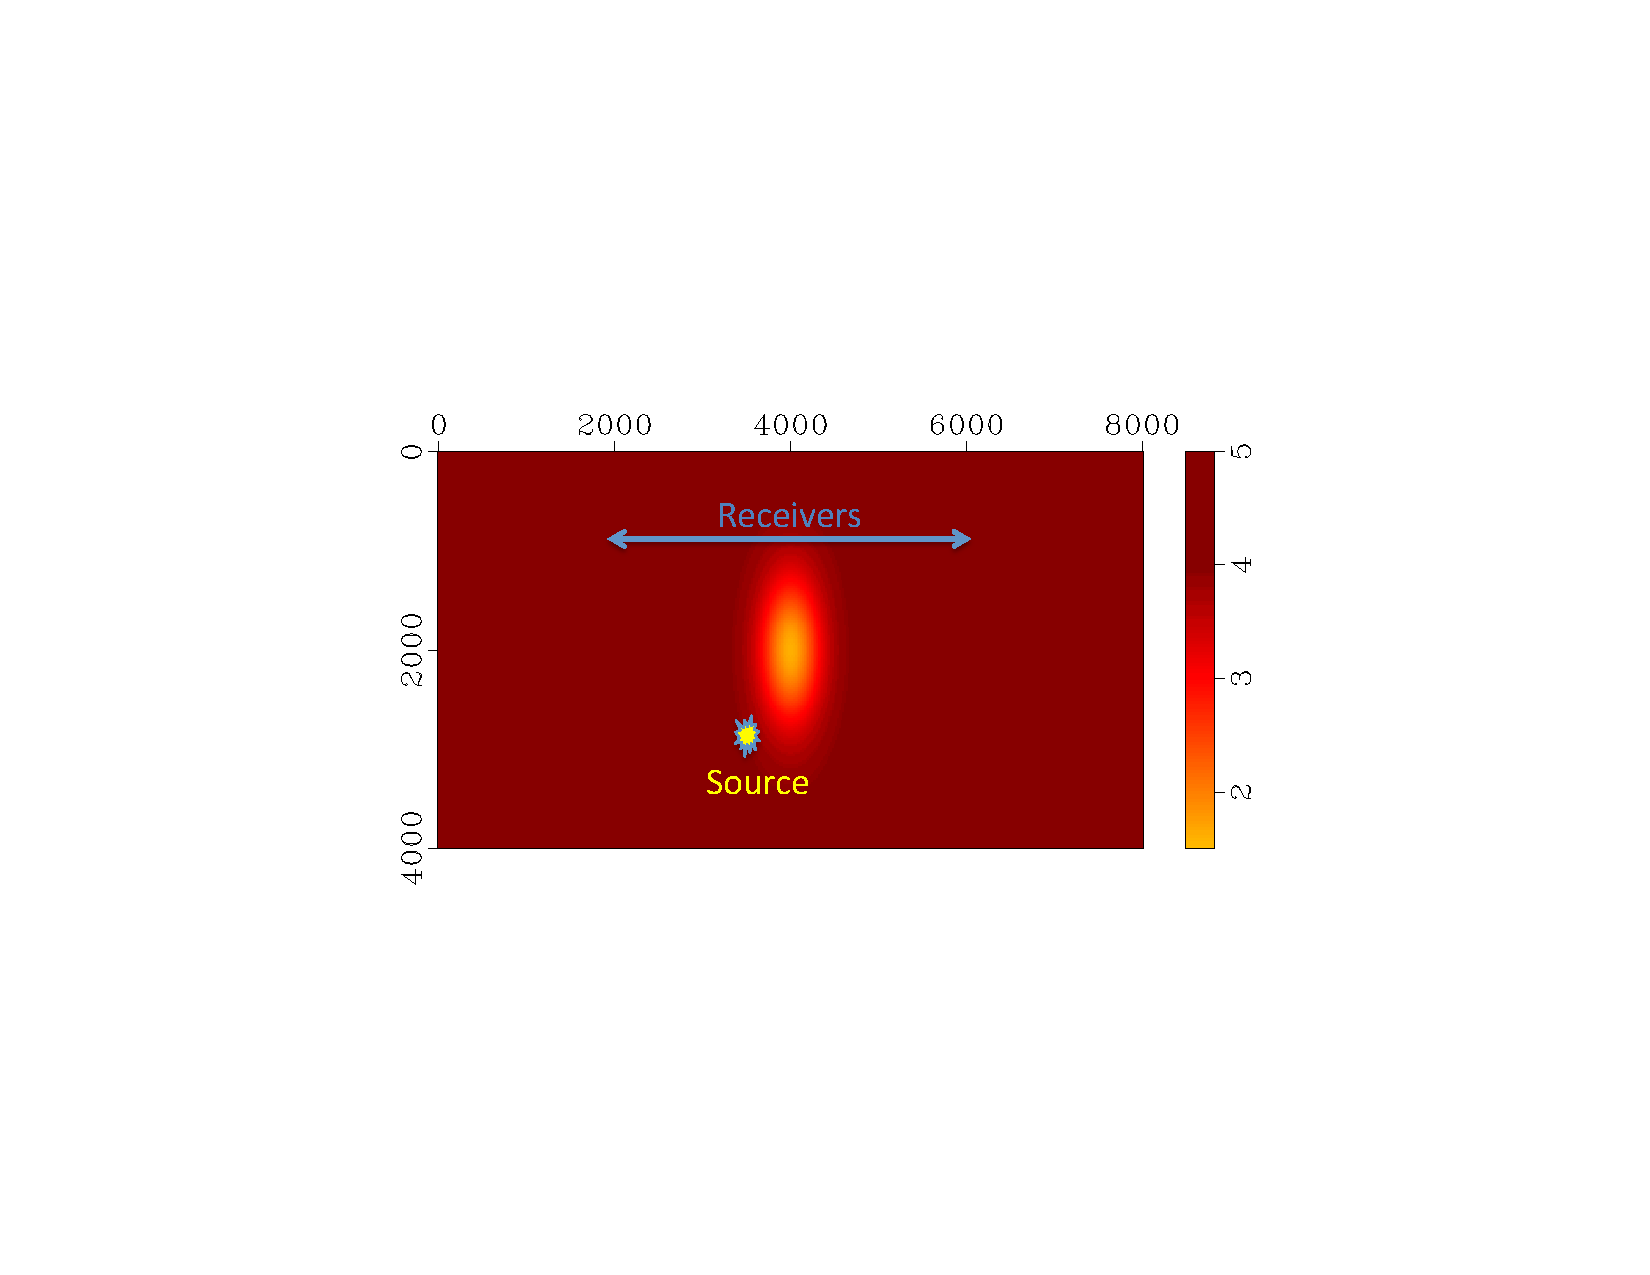
\includegraphics[height=4.0in]{Fig/bml0c.pdf}\\
%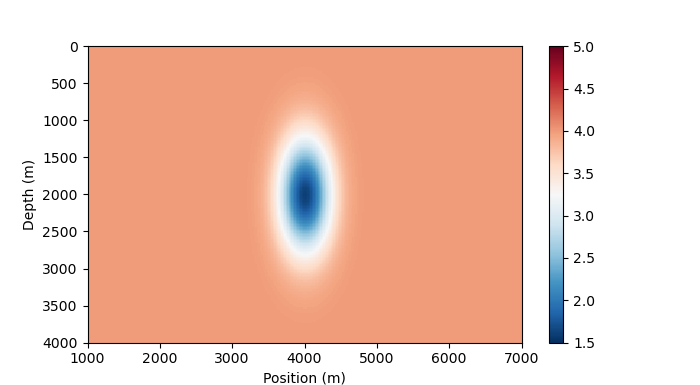
\includegraphics[height=2.0in}{Fig/bml0.pdf}\\
\begin{center}
\vspace{0.25in}
\includegraphics[height=1.25in]{Fig/bml0.png}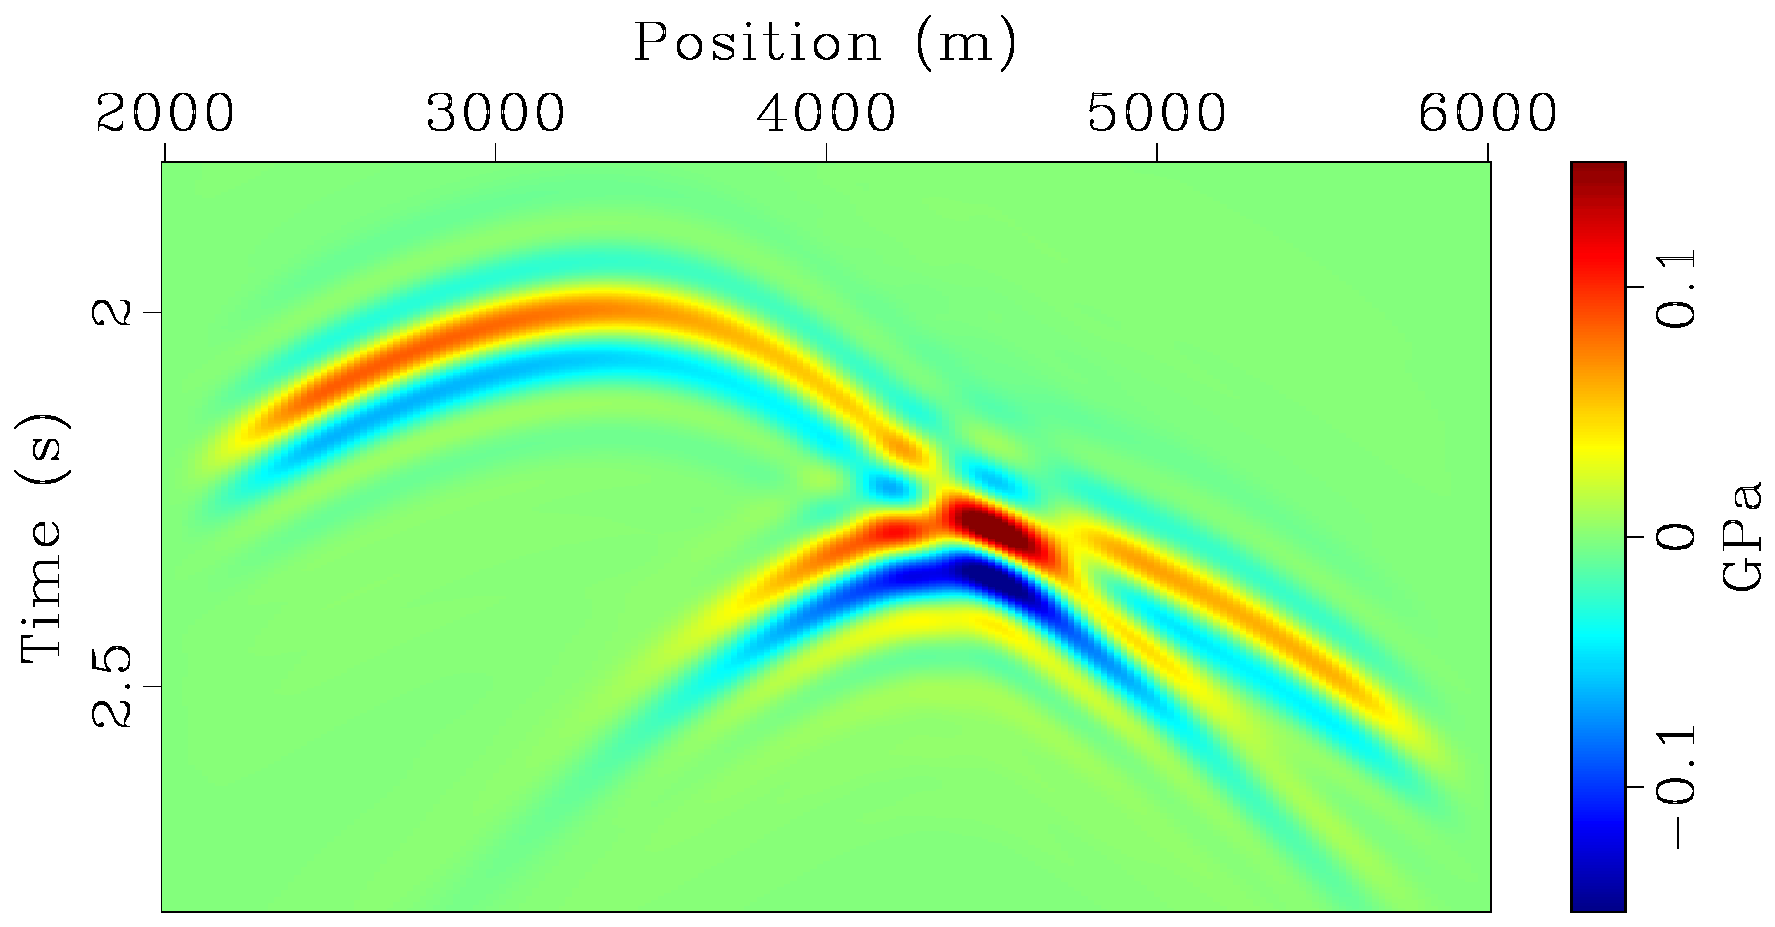
\includegraphics[height=1.25in]{Fig/ptpwindl0.pdf}\\
\vspace{0.5cm} Left: target bulk modulus $\kappa$, source at
$x_s=3500$ m, $z_s=3000$ m, receivers at $x_r=2000-6000$ m, $z_r=1000$
m. Right: synthetic data, source pulse = [1.0, 2.0, 7.5, 12.5] Hz trapzoidal bandpass filter]
\end{center}
\end{frame}

%\begin{frame}
%Modeling operator $(S[\kappa]f)(t,x_r) = \phi(x_r) p(t,x_r,z_r)$ - linear in $f$, nonlinear in $\kappa$
%Model $m=[\kappa]$, wavefield $u=[p,\bv]$, $L[m]u=$ acoustic wave system, $R$ = sample $p$ at receivers, 
%\begin{center}
%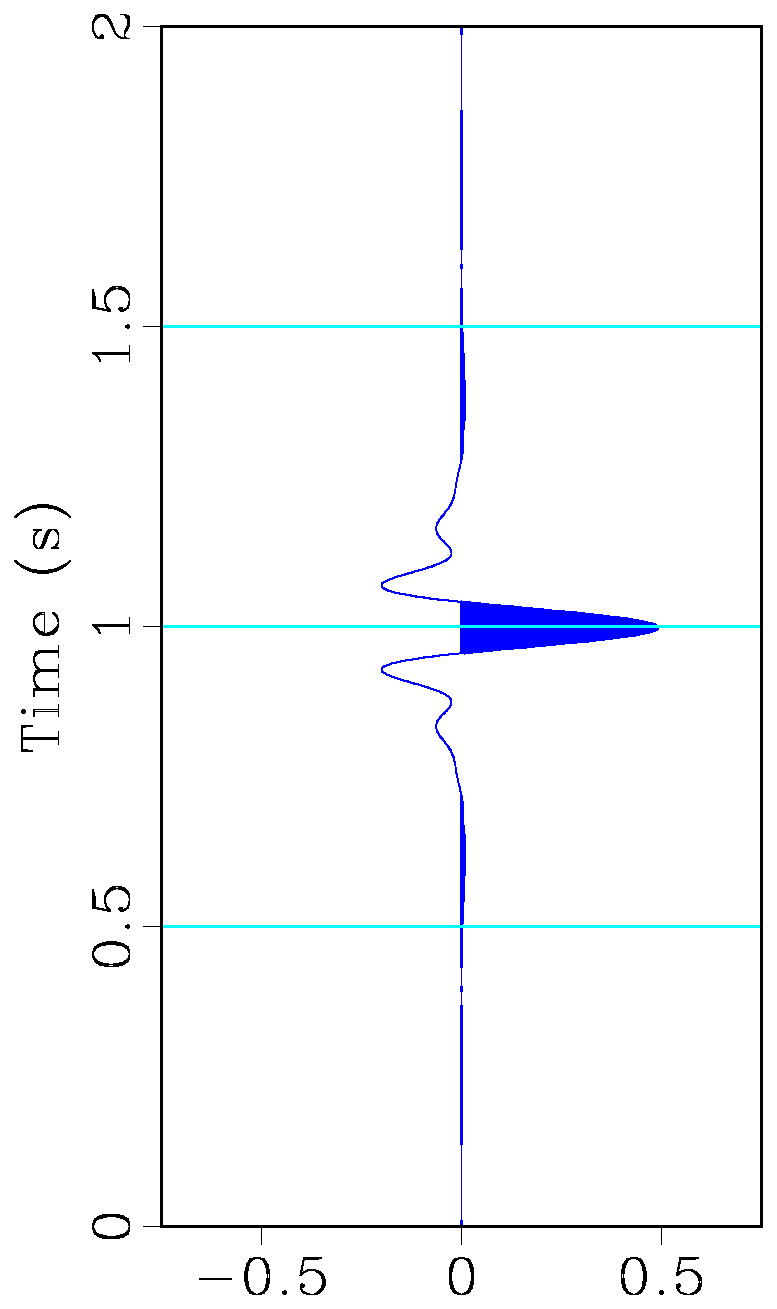
\includegraphics[height=1.5in]{Fig/pulse00.pdf} 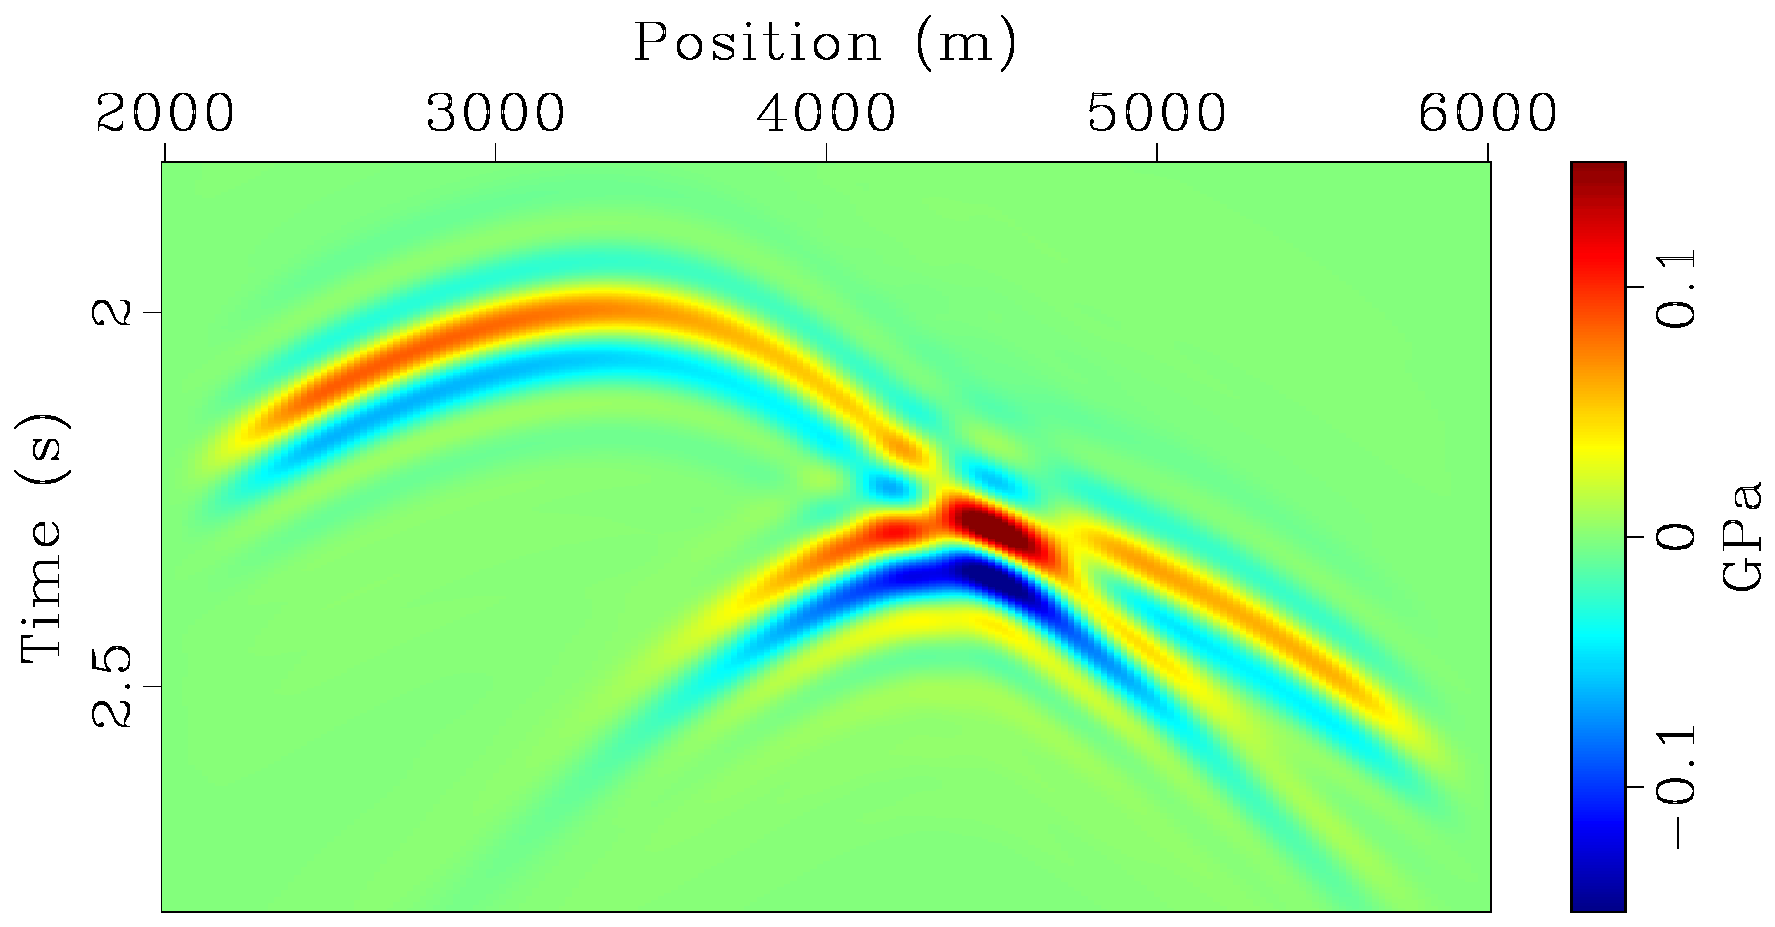
\includegraphics[height=1.5in]{Fig/ptpwindl0.pdf}\\
%\vspace{0.25in}
%Left: [1.0, 2.0, 7.5, 12.5] Hz trapzoidal bandpass filter pulse $w$; Right: pressure traces $Ru$ at $z_r=1000 m$ for source at $x_s=3500 m, z_s=3000 m$. 
%\end{center}
%\end{frame}

\begin{frame}
\begin{center}
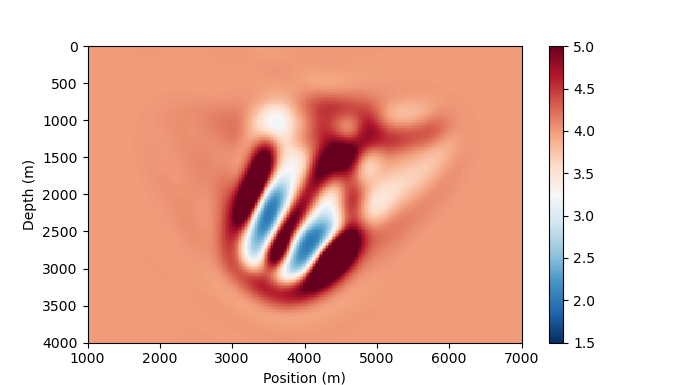
\includegraphics[height=1.25in]{Fig/covmestfwi2.png}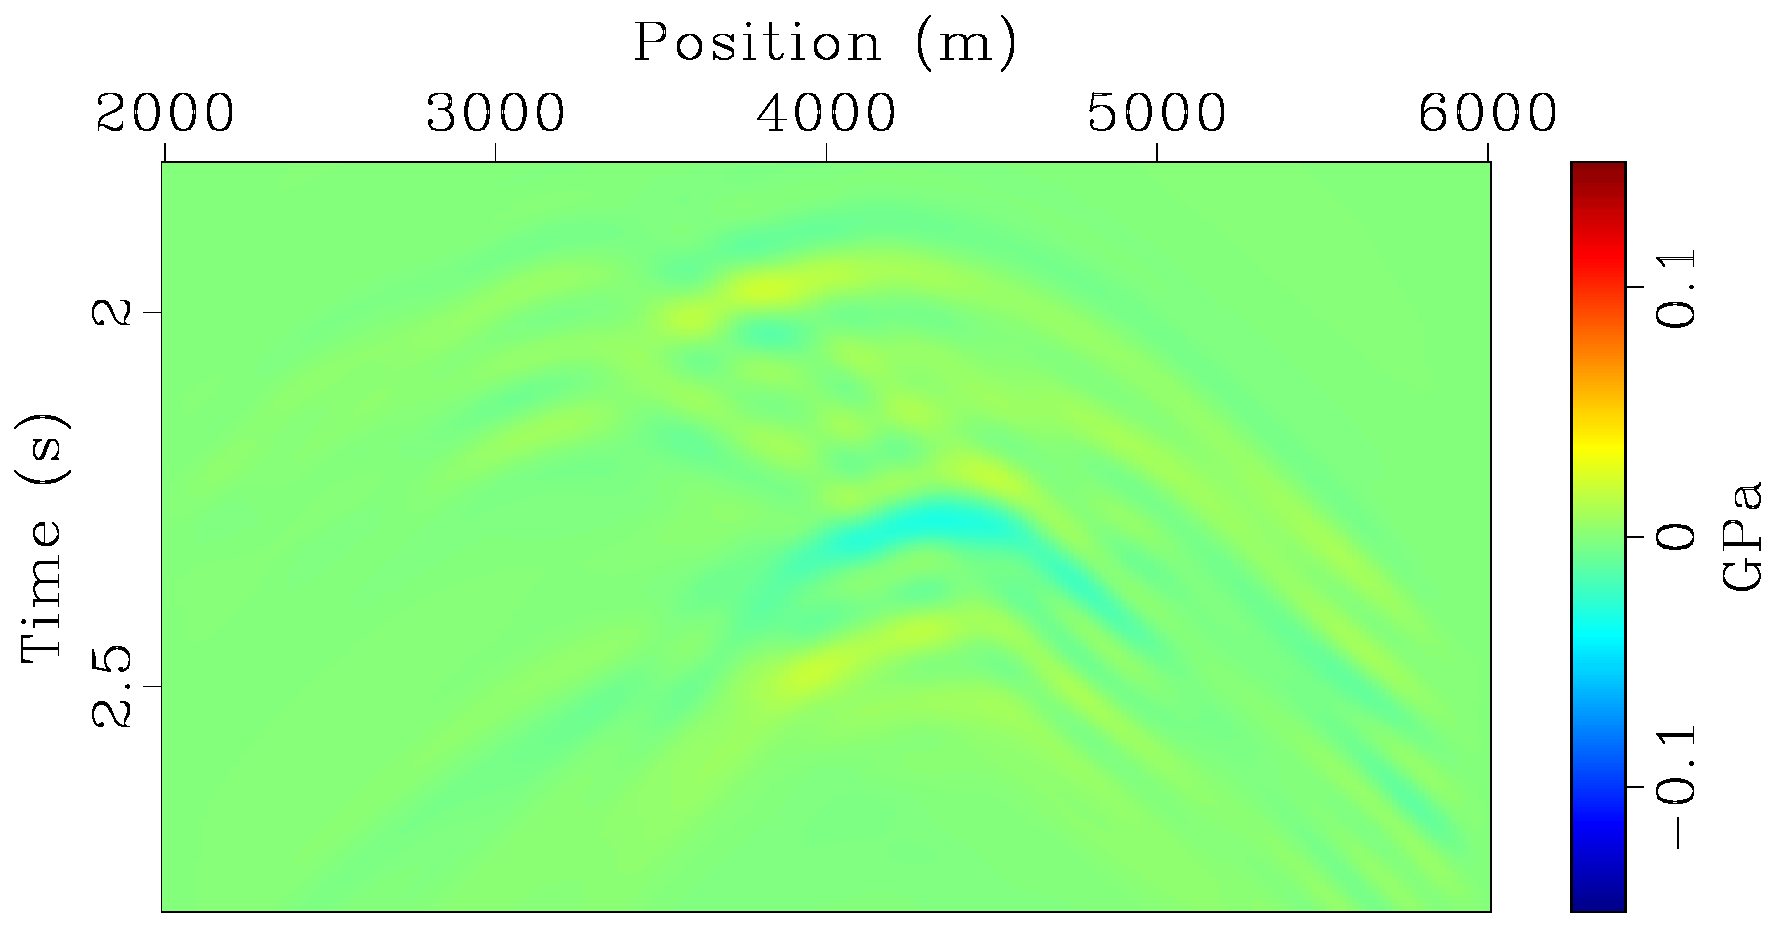
\includegraphics[height=1.25in]{Fig/residcovmestfwi2wind.pdf}\\
\vspace{0.5cm}
Left: target model; 
Right: FWI estimate of $m$ = bulk modulus: initial model $\kappa_0
\equiv 4.0$ GPa, 450 steps steepest descent with smoothing
preconditioner. Right: data residual ($Ru - d$) - energy (norm)
$\approx 25$\% of data norm.
\end{center}

Failure mechanism: ``cycle skipping'', first documented in Gauthier-
\textcolor{blue}{Virieux}-Tarantola 86 - half-wavelength
criterion, (\textcolor{blue}{Virieux}-Operto 09)
\end{frame}



%\begin{frame}
%\begin{center}
%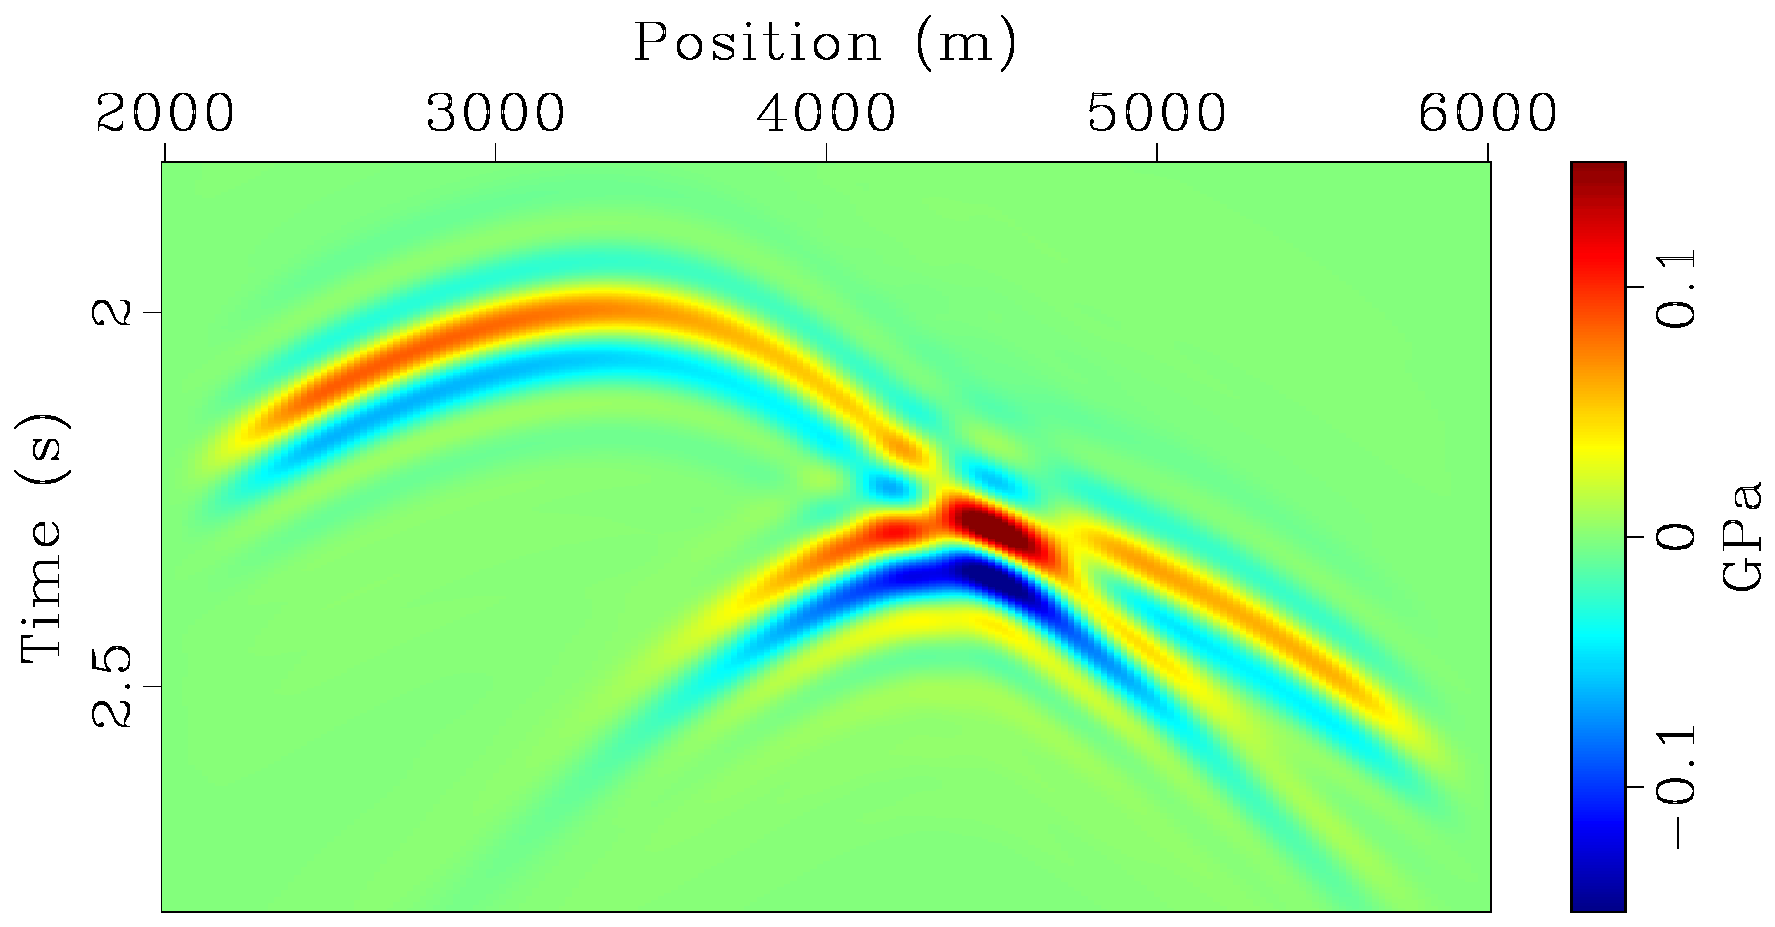
\includegraphics[height=1.2in]{Fig/ptpwindl0.pdf}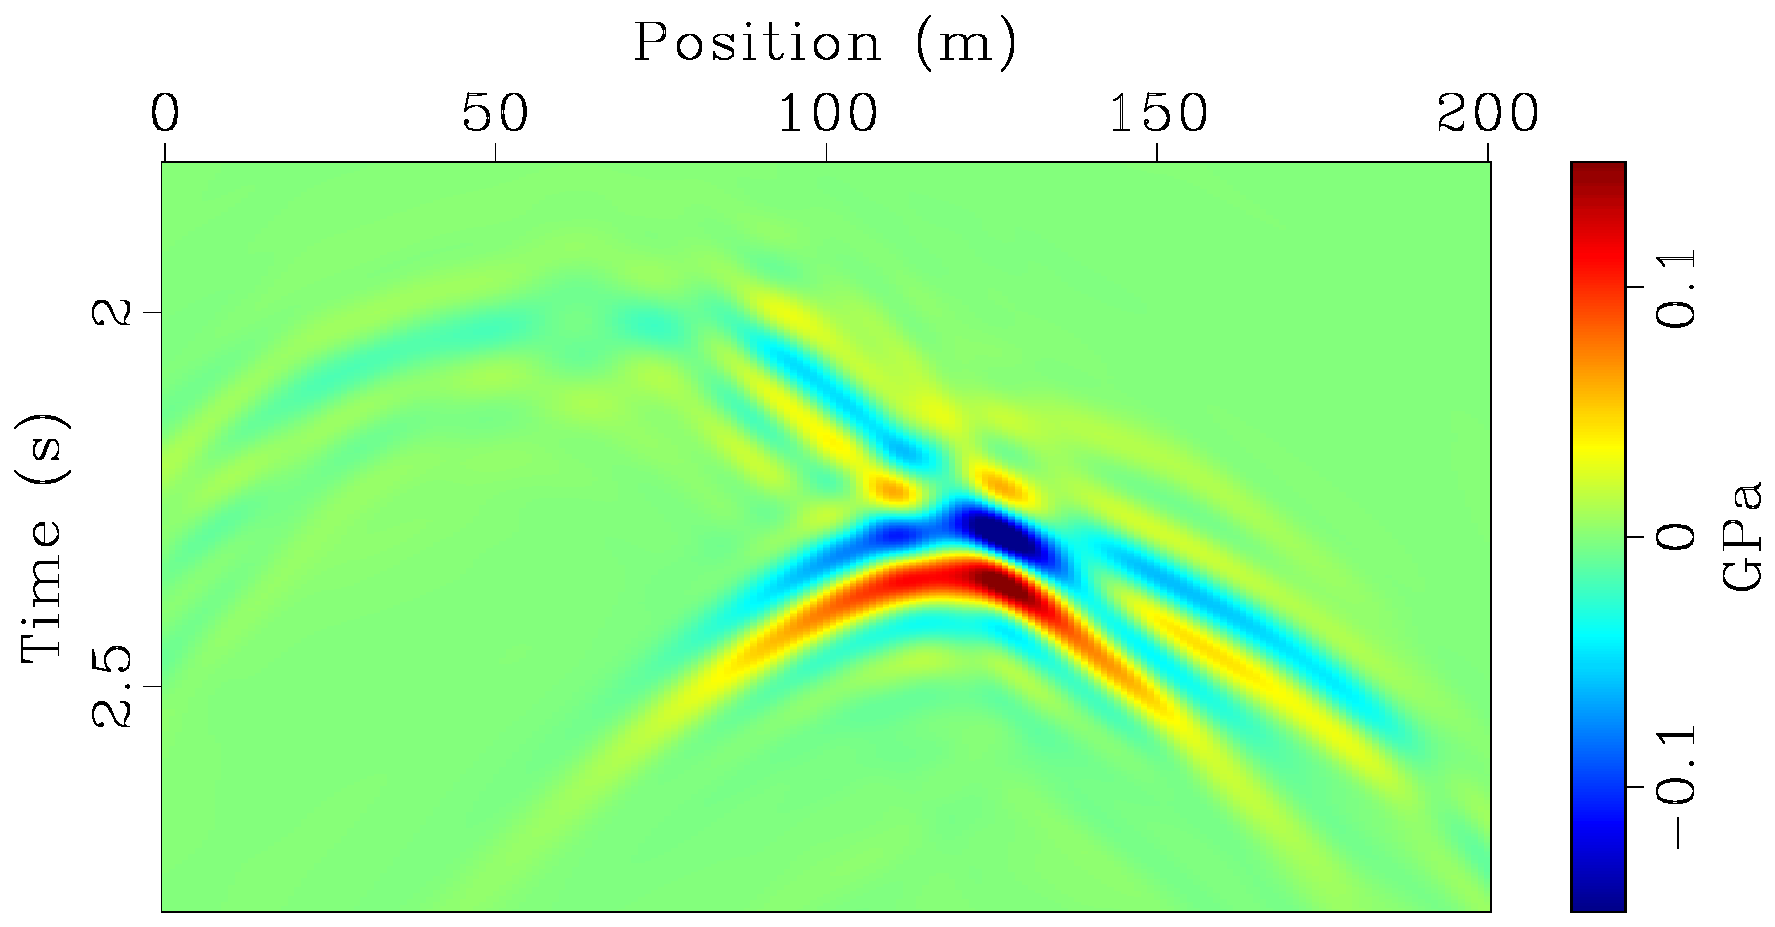
\includegraphics[height=1.2in]{Fig/fwitrreslh0wind.pdf}\\
%\vspace{0.5cm}
%Left: target data; 
%Right: data residual after 20 KGN steps - final RMS residual reduction = 0.26
%\|d\|=9.72 \|S-d\|=2.51
%\end{center}
%\end{frame}


%\begin{frame}
%Big problem: "cycle skipping"
%\begin{itemize}
%\item $J[m]$ appears to have many (local) minima
%\item to avoid getting stuck at wrong estimates, initial $m$ (and $f$) must predict eve%nt times in $u$ ``correct within a wavelength''
%\end{itemize}

%OK with sufficiently low frequency data with high S/N, but not always available
%\end{frame}

\section{Extension}
\begin{frame}
  Many proposed cures for cycle skipping:
  \begin{itemize}
  \item acquire lower frequency data (Dellinger et al SEG 2016,...) 
  \item combine with traveltime tomography (Luo-Schuster 91,
    Prieux-\ldots-\textcolor{blue}{Virieux} 13)
  \item use a different objective, e.g. transport metric
    (Yang-Engquist 18, M\'{e}tivier-...-\textcolor{blue}{Virieux} 18)
  \item use a different model - {\em enlarge search space, easier data
    fit} (``model extension'')
  \end{itemize}

Many extension methods - Operto et al. 23, Farshad-Chauris 23, Huang
et al 19, S. 08. Common theme: maintain data fit while suppressing
additional degrees of freedom
\end{frame}


\begin{frame}
  \vspace{0.25in}
Example: Adaptive Waveform Inversion (AWI, Warner-Guasch 14): acoustic
model, {\em known} isotropic point source $s = w(t)\delta(\bx-\bx_s)$,

Idea: if events in predicted data $F[m]s$ are in wrong place, use a 
filter $f$ to put them in the right place: extended modeling op $\bar{F}[m,f] = f*F[m]$.
\vspace{-0.25in}
\begin{center}
  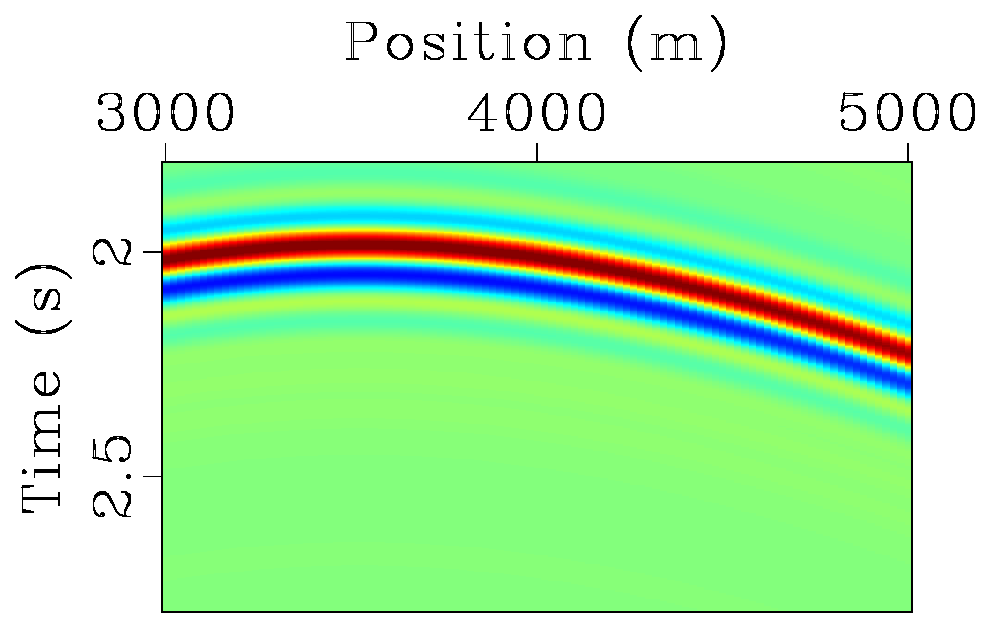
\includegraphics[height=1in]{Fig/ptph0half.pdf}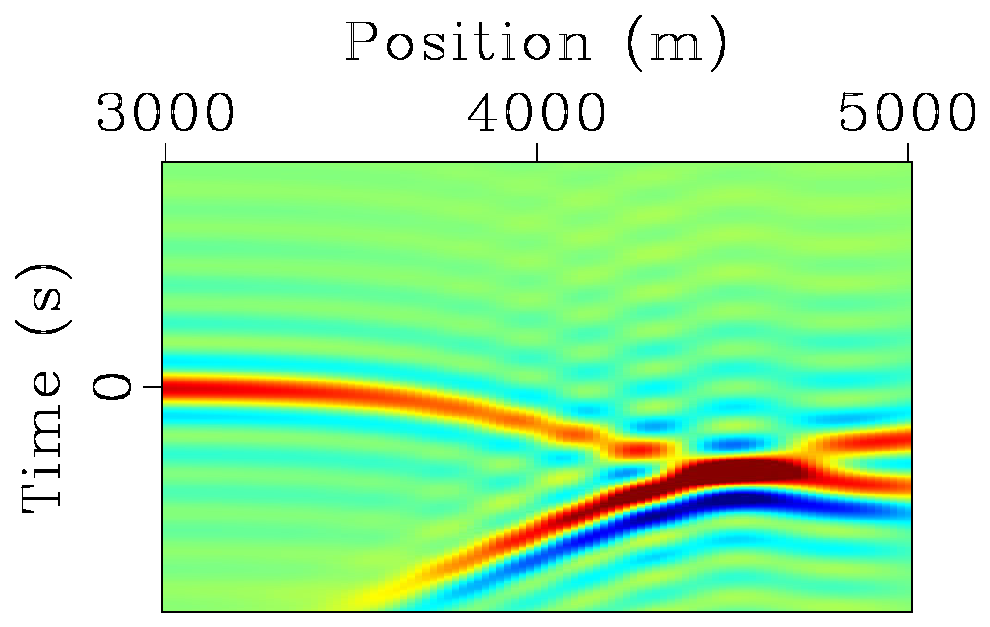
\includegraphics[height=1in]{Fig/uest0half.pdf}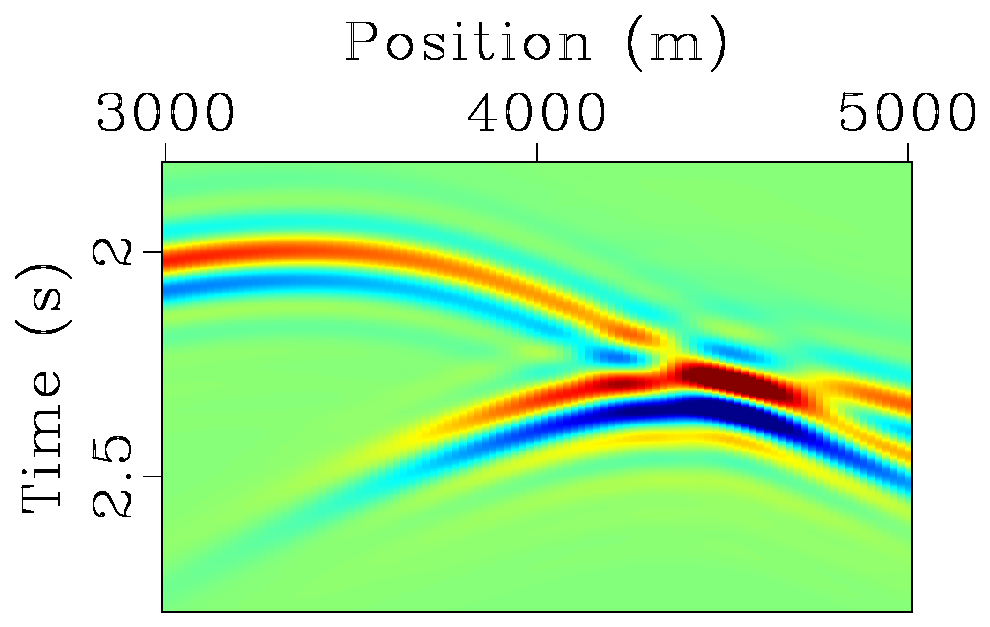
\includegraphics[height=1in]{Fig/ptpl0half.pdf}\\
\vspace{0.5cm}
Left: Predicted data $F[m_0]s$, $m_0=$ homogenous model; Center: adaptive filter $f$;
Right: adapted data $f*F[m_0]s \approx d =$ lens data
\end{center}

\end{frame}
\begin{frame}
$f$ = $d$ deconvolved (trace-by-trace) by $F[m]s$ (``easy''), so can
make $\bar{F}[m,f]s$ fit data {\em for any m} (common feature of extension methods)

but $\bar{F}[m,f] \ne F[m]$ unless $f(\bx_s,\bx_r,t)=\delta(t)$ - to
test, find an operator vanishing on $\delta(t)$ (``annihilator'' -
another common feature), update $m$ to reduce its output

$t\delta(t)=0$, so minimize
\[
J_{\rm AWI}[m] = \sum_{\bx_s,\bx_r}\frac{{\sum_t|\color{blue}t}
  f[m](\bx_s,\bx_r,t)|^2}{\sum_{t}| f[m](\bx_s,\bx_r,t)|^2}
\]
\end{frame}

%\begin{frame}
%\vspace{-1in}
%\begin{center}
%\hspace{-0.5in}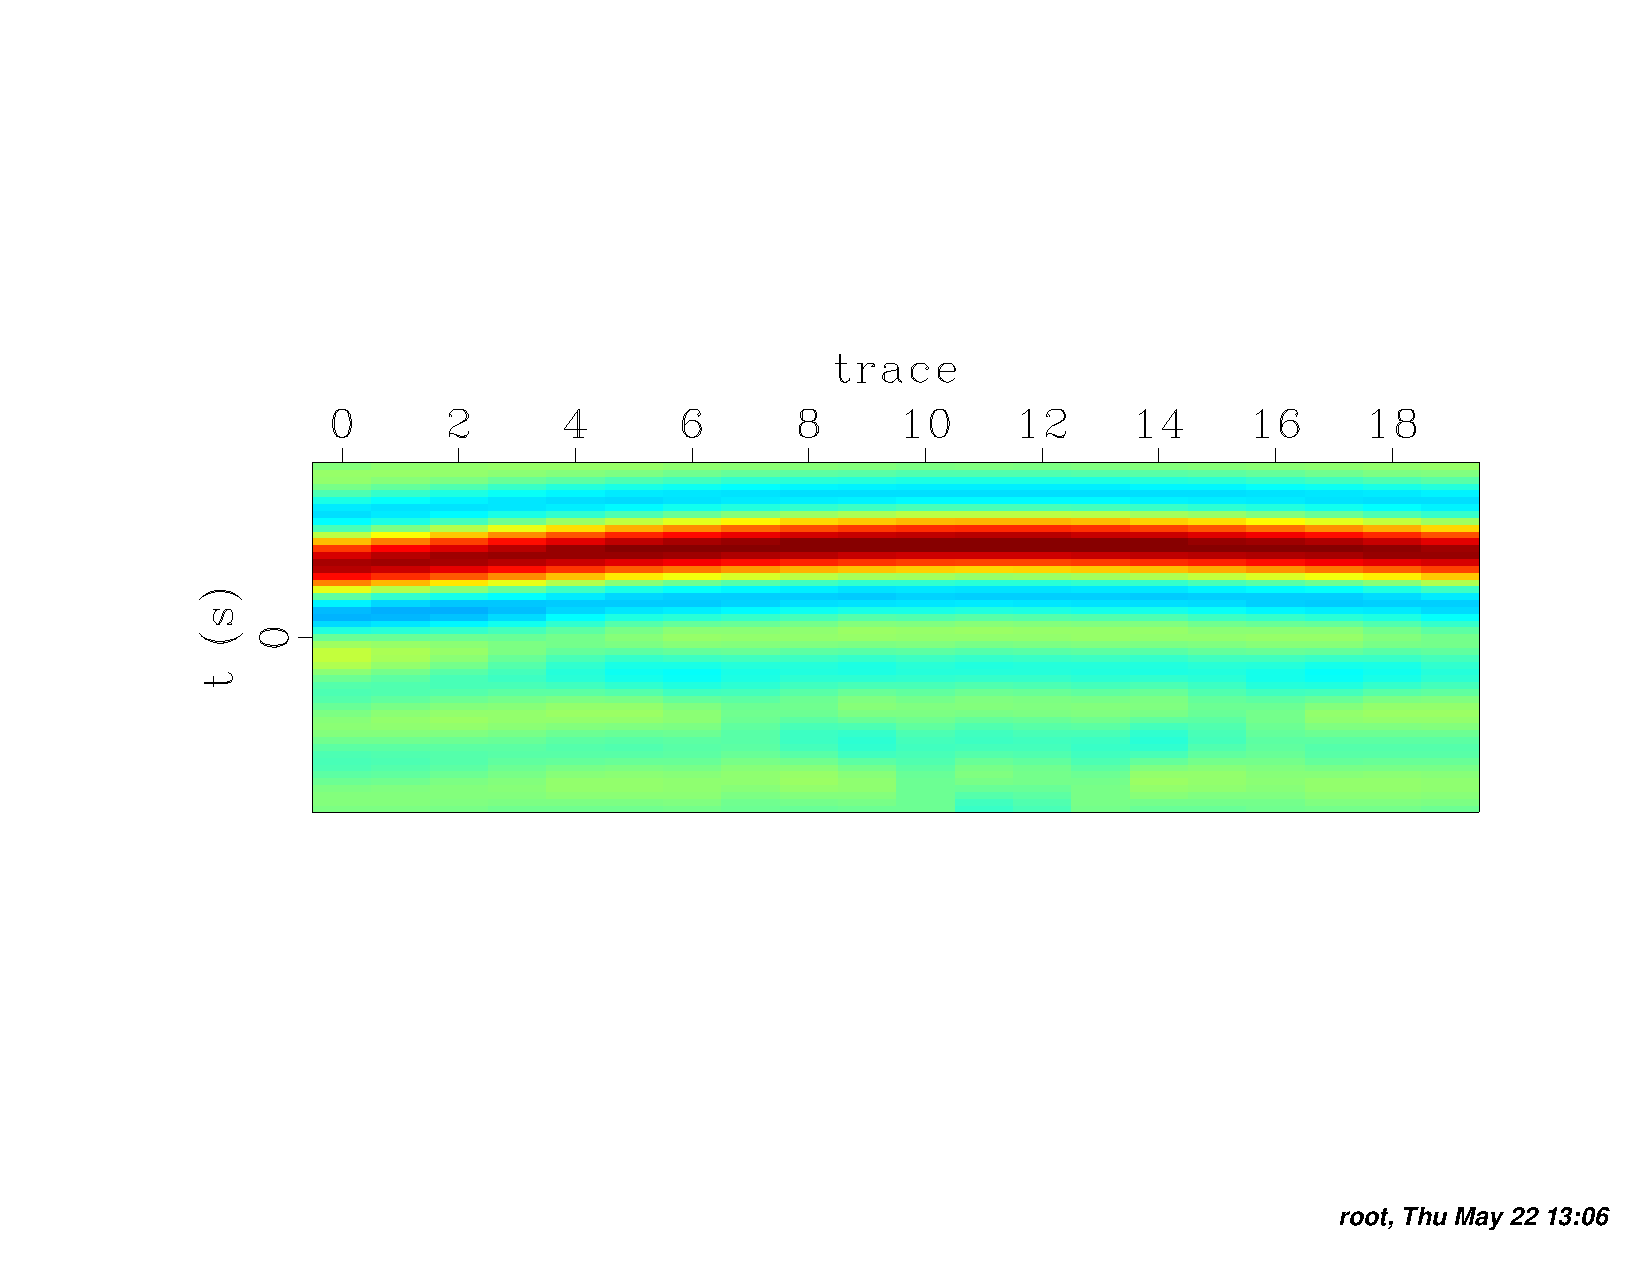
\includegraphics[height=2.5in]{Fig/uest0gz1800wind.pdf}\hspace{-0.5in}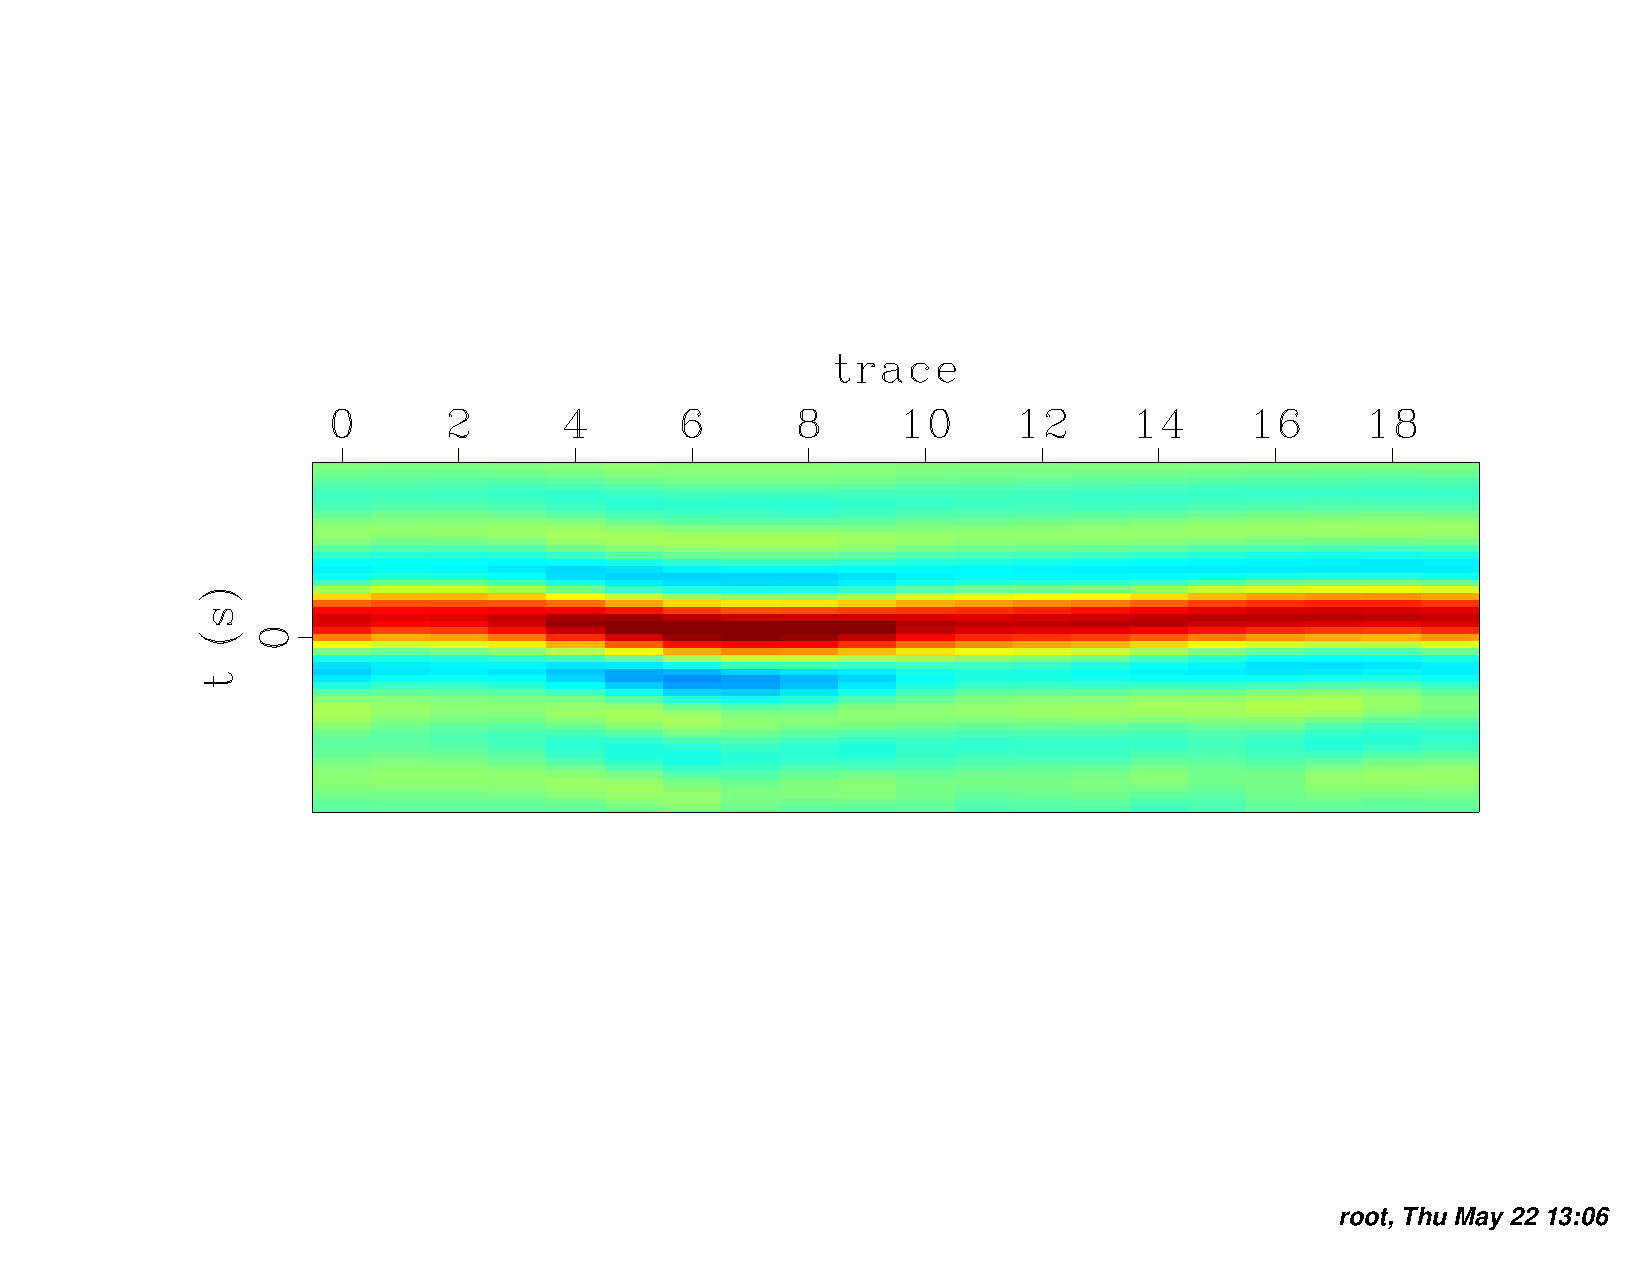
\includegraphics[height=2.5in]{Fig/uestmswigz1800wind.pdf}\\
%\vspace{-0.75in}
%Left: $f[m]$, $m$=initial model. Right: $f[m]$, $m$ updated to reduce
%$J_{\rm AWI}$
%\end{center}
%\end{frame}

\begin{frame}
  Good News: suppose
  \begin{itemize}
  \item transmission data dominated by single arrivals - unique
    travel time $\tau$ between source and receiver,
  \item $d \approx F[m_*]s$
  \item RMS wavelength of $w \rightarrow 0$.
  \end{itemize}
  Then
  \[
    J_{\rm AWI}[m] \rightarrow \sum_{\bx_s,\bx_r} |\tau[m]-\tau[m_*]|^2
  \]

  \textcolor{blue}{For single-arrival data, AWI is asymptotic to
    travel time tomography} $\Rightarrow$ no cycle-skipping

  \end{frame}

  \section{Triplication}

\begin{frame}
  Conclusion does not apply to acoustic lens example - multiple
  arrivals.

  Asymptotic analysis, numerical examples $\Rightarrow$

  Significant energy in $d$ at multiple arrival times $\Rightarrow$
  approach based on source-receiver extension (e. g. AWI) behaves like
  FWI (S. 94, Plessix et al. 00, Huang et al. 17, Yong et al. 23.)

\begin{center}
\hspace{-0.5in}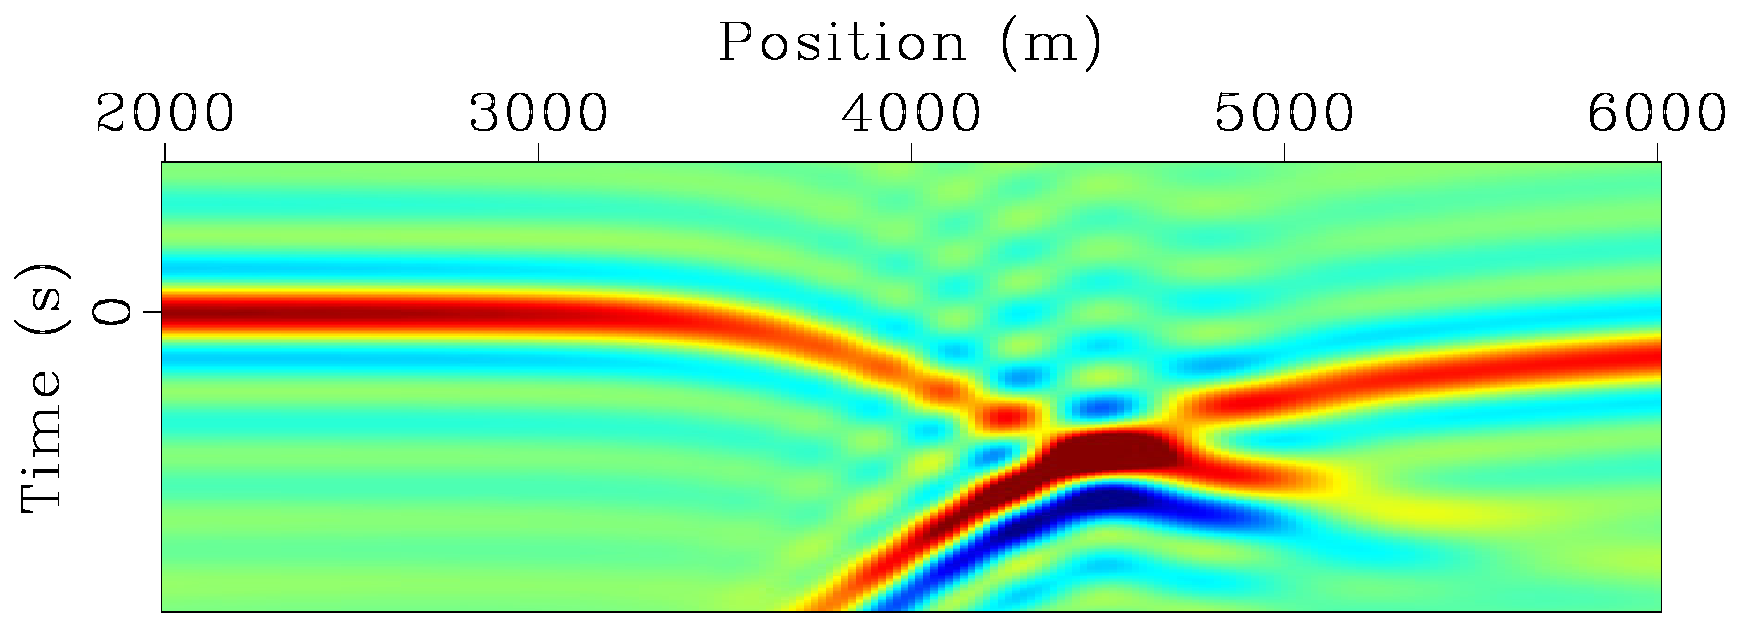
\includegraphics[height=0.8in]{Fig/uest0wind.pdf}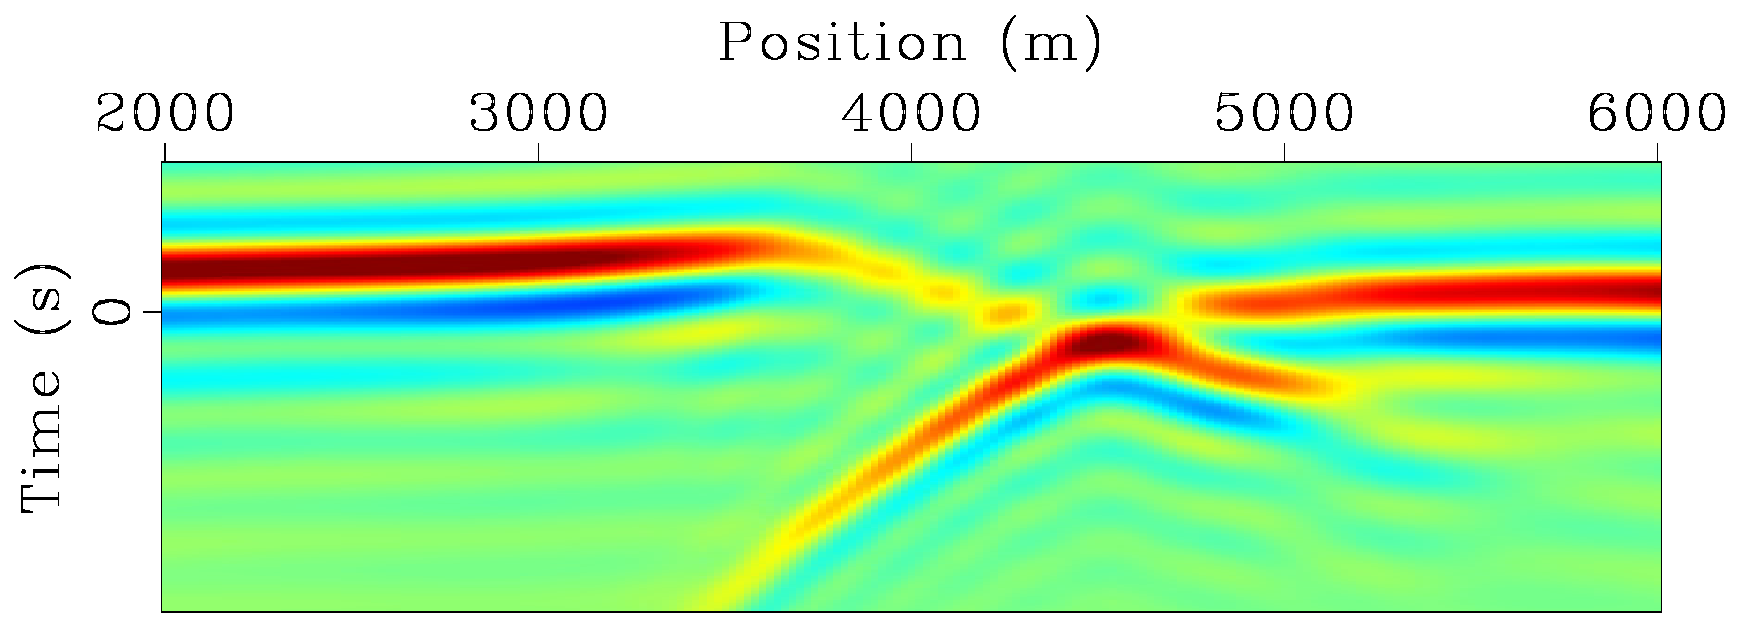
\includegraphics[height=0.8in]{Fig/uestmswiwind.pdf}\\

Adaptive filters for lens data. Left: $f[m]$, $m$=initial model. Right: $f[m]$, $m$ updated to reduce
$J_{\rm MSWI}$ (similar to $J_{\rm AWI}$).
\end{center}
\end{frame}

\begin{frame}
  Remedy: localize inversion around individual events

  \begin{itemize}
  \item localize in time - Yong-Brossier-Métivier-\textcolor{blue}{Virieux} 23: Local
    Adaptive Waveform Inversion (LAWI) via Gabor filter
  \item localize in phase space - surface source extension (SSE) -
    Huang et al. 19
  \end{itemize}

  SSE extended source: $\bar{s} = \bar{w}(\bx,t;\bx_s)\delta_{{\cal
      S}}(\bx)$, ${\cal S} $= surface containing source locations -
  {\em spread source energy over a surface}, acts as antennae,
  controls full 2D phase spectrum

For any $m$, determine $\bar{w}=\bar{w}[m]$ so that $F\bar{s} \approx d$. Update $m$ to drive
$\bar{w}(\bx,t;\bx_s) \rightarrow w(t)\delta(\bx-\bx_s)$ by minimizing
\[
  J_{\rm SSE}[m] = \sum_{\bx_s}\sum_{\bx,t} ||(\bx-\bx_s)|
  \bar{w}[m](\bx,t;\bx_s)|^2
 \]
\end{frame}


  
    





%\begin{frame}
%Detailed Formulation:

%At solution, must recover known constraints on model (``get closer to Vancouver's latitude as you get close to the sea''): 

%$\Rightarrow$ introduce {\color{blue} annihilator} $A$, vanishing on models obeying these constraints - minimize output jointly with data residual

%Many possibilities - MS difference w/ known source (WRI), mean time lag (AWI)

%Many choices. For SSE: scale by offset 
%\[
%A\of(\bx,t;x_s,y_s) = \sqrt{(x-x_s)^2+(y-y_s)^2}w(x,y,t;x_s,y_s)
%\]

%{\color {blue} Extension Principle:} $m,\of$ so  that $R\bar{u} \approx d$, $A\of \approx 0$ $\Rightarrow$ approx FWI solution
%\end{frame}



%\begin{frame}
%Extended objective function: data misfit + annihilator output, 

%\[
%J_{\rm SSE}[m] = \min_{\of} \,\frac{1}{2} \sum (R\ou - d)^2 + \alpha^2 \sum (A\of)^2
%\]

%Reduced: ``pre-minimized'' over source

%FWI via surface source extension: given $d$ and initial $m_0$, use numerical optimization method to find minimizer $m$ of
%$J_{\rm SSE}[m]$.
%\end{frame}

%\begin{frame}
%Examples: 

%(1) diving wave data (sampling op may include window in defn)

%(2) reflection data

%In both cases, method is [??? VPM, CG for inner problem, steepest descent for outer???]
%\end{frame}

%\begin{frame}
%Mohamed's examples 
%\begin{itemize}
%\item include straight FWI for both
%\item also some info about objective values, residuals, convergence, etc.
%\item plots of models, but also sources, residuals - especially want to show extended source from early iteration
%\end{itemize}
%\end{frame}

\begin{frame}
Penalty method: minimize
\[
J_{\alpha}[m,\bar{w}] = \frac{1}{2} \sum |F[m]\bar{w} - d|^2 + \alpha^2||\bx-\bx_s|\bar{w}|^2
\]
over $m$ 

\begin{itemize}
\item time-domain FD, gradient via adjoint state
\item Variable Projection:
  \begin{itemize}
  \item update $\bar{w}$ using Conjugate Gradient Iteration (inner loop)
\item update $m$ using steepest descent, line search (outer loop) plus
  smoothing regularization
  \end{itemize}
\item update $\alpha$ using Discrepancy Principle (keep data residual $\in (e_-, e_+)$) - {\color{blue} can always choose $\bar{w}$ to fit data} $\Rightarrow$ can start with $\alpha=0$ (Fu \& S. 17)
\end{itemize}
\end{frame}

\begin{frame}
\begin{center}
SSE for 1 shot lens data, source surface ${\cal S} = \{z = 3000 m\}$
\end{center}
\begin{center}
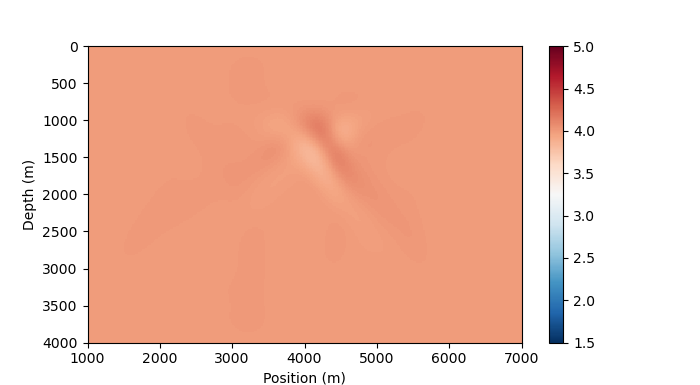
\includegraphics[height=1.25in]{Fig/cgw1_bulkupdlh0.png}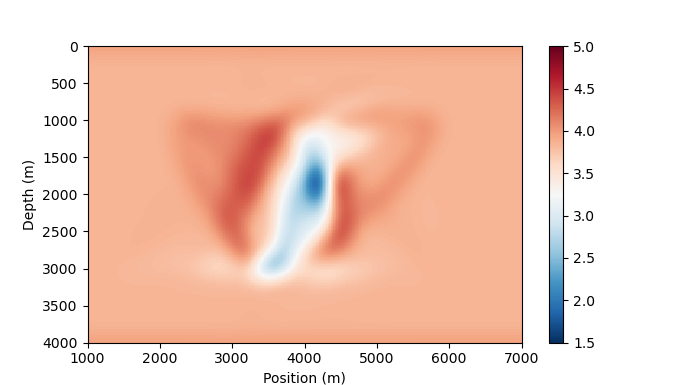
\includegraphics[height=1.25in]{Fig/cgw41_bulkupdlh0.png}\\
\vspace{0.25in}
Start at $\kappa_0=4.0$ GPa, use $e_-=0.05\|d\|, e_+=0.1\|d\|$. \\
Left: Iteration 1 ($\alpha=2.9 e-6$)\\
Right: Iteration 41 ($\alpha = 1.99 e-5$)
\end{center}
\end{frame}

\begin{frame}
$m=[\kappa]$ converges $\leftrightarrow$ $\alpha$ increases, extended source $\of$ (initially spread over $z=z_s=3000$ m) {\color{blue} focuses} at $x=x_s=3500$ m.
\begin{center}
\hspace{-1cm}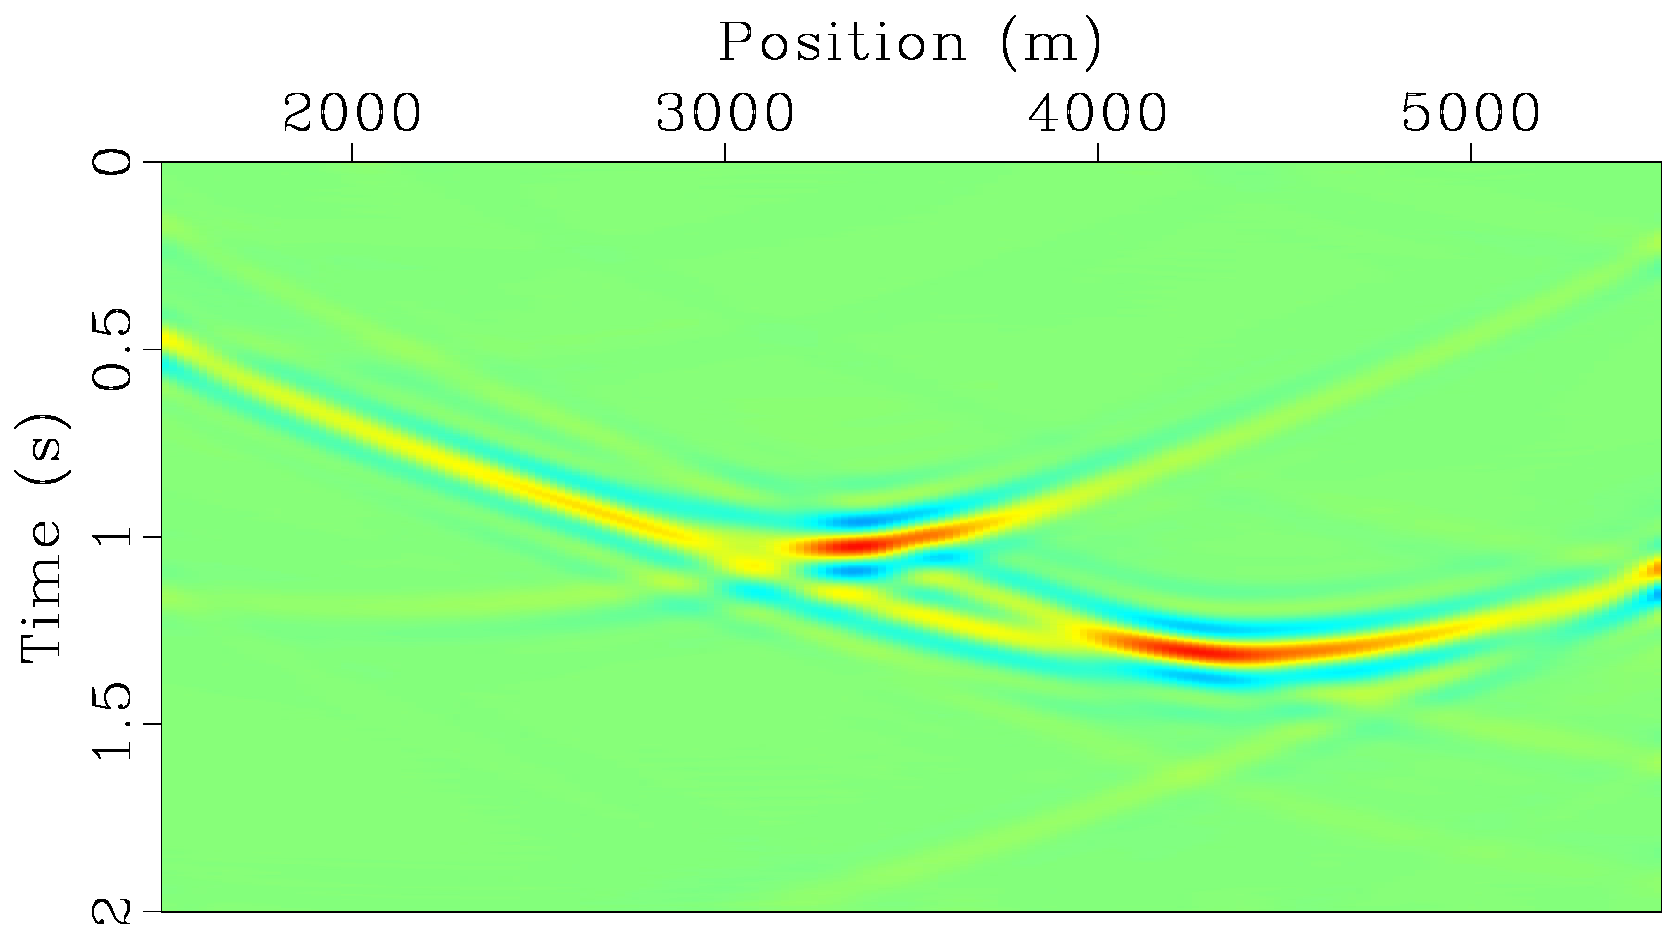
\includegraphics[height=1.25in]{Fig/cgw0_est_source_plh0.pdf}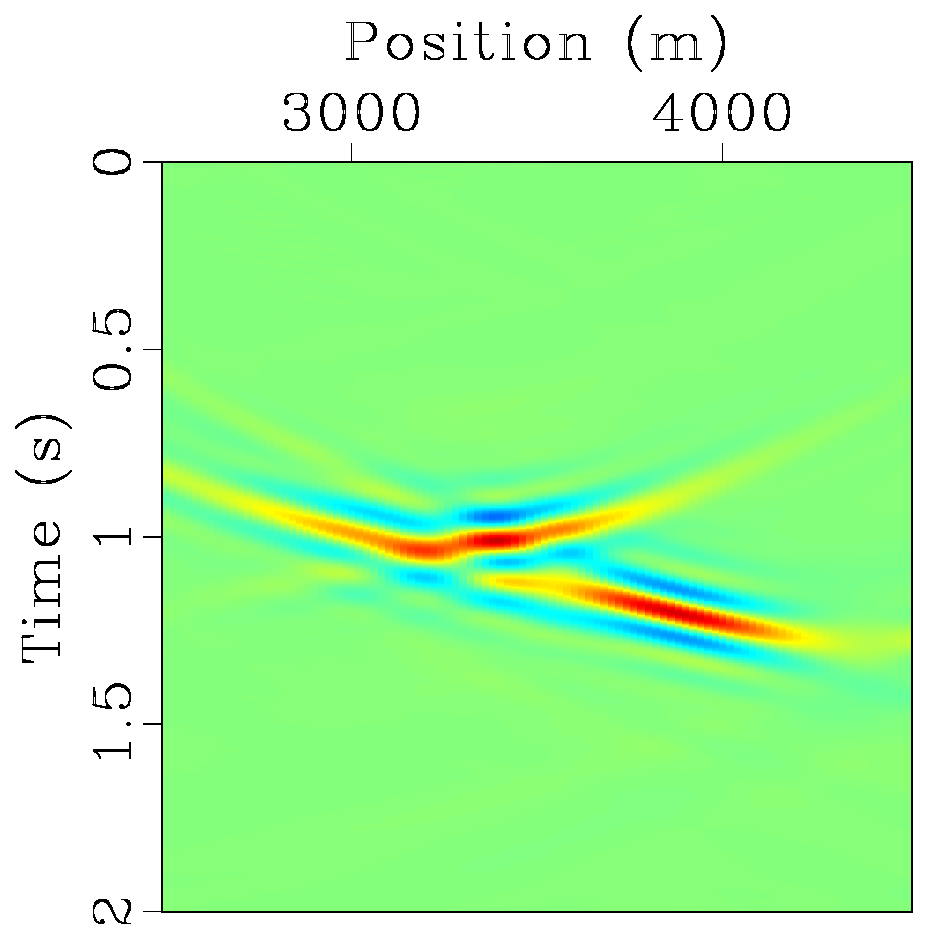
\includegraphics[height=1.25in]{Fig/cgw8_est_source_plh0.pdf}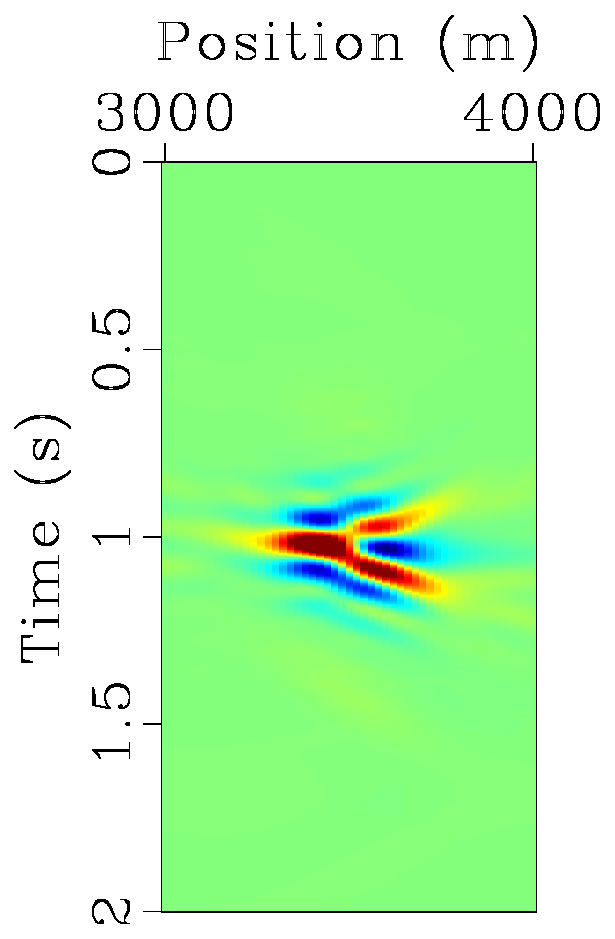
\includegraphics[height=1.25in]{Fig/cgw18_est_source_plh0.pdf}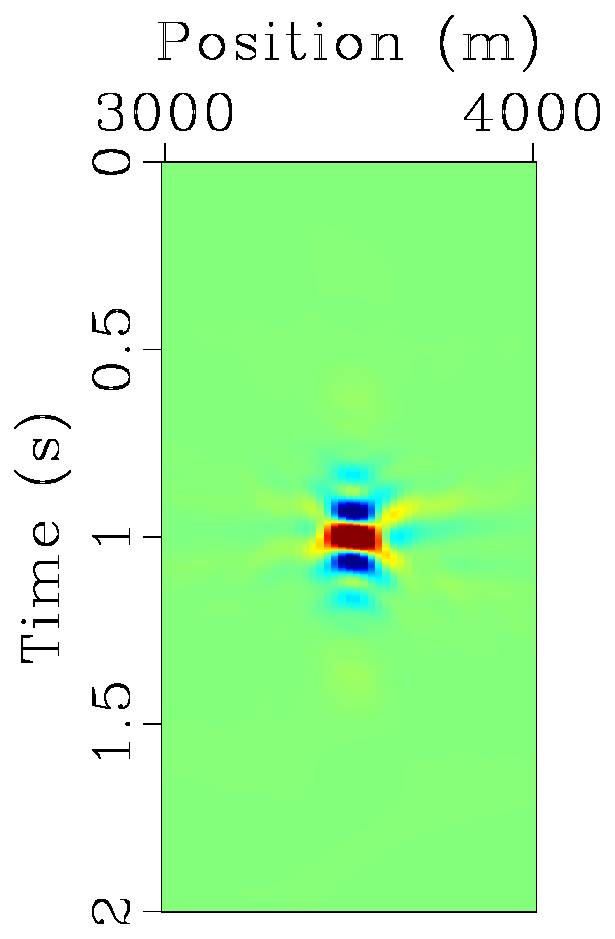
\includegraphics[height=1.25in]{Fig/cgw40_est_source_plh0.pdf}\\
\vspace{0.25in}
Left to right: $\of$ at Iterations 1 ($\alpha=2.9 e-6$), 9
($\alpha= 5.2 e-6$ m) 19 ($\alpha=1.32 e-5$) and 41 ($\alpha=1.99e-5$).
\end{center}
\end{frame}

\begin{frame}
\begin{center}
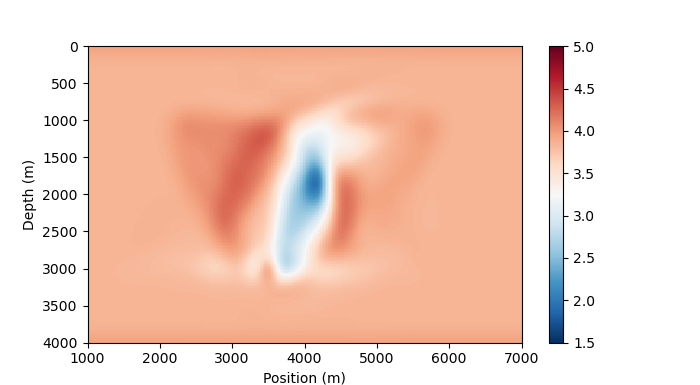
\includegraphics[height=1.25in]{Fig/covmestfwicgw41.png}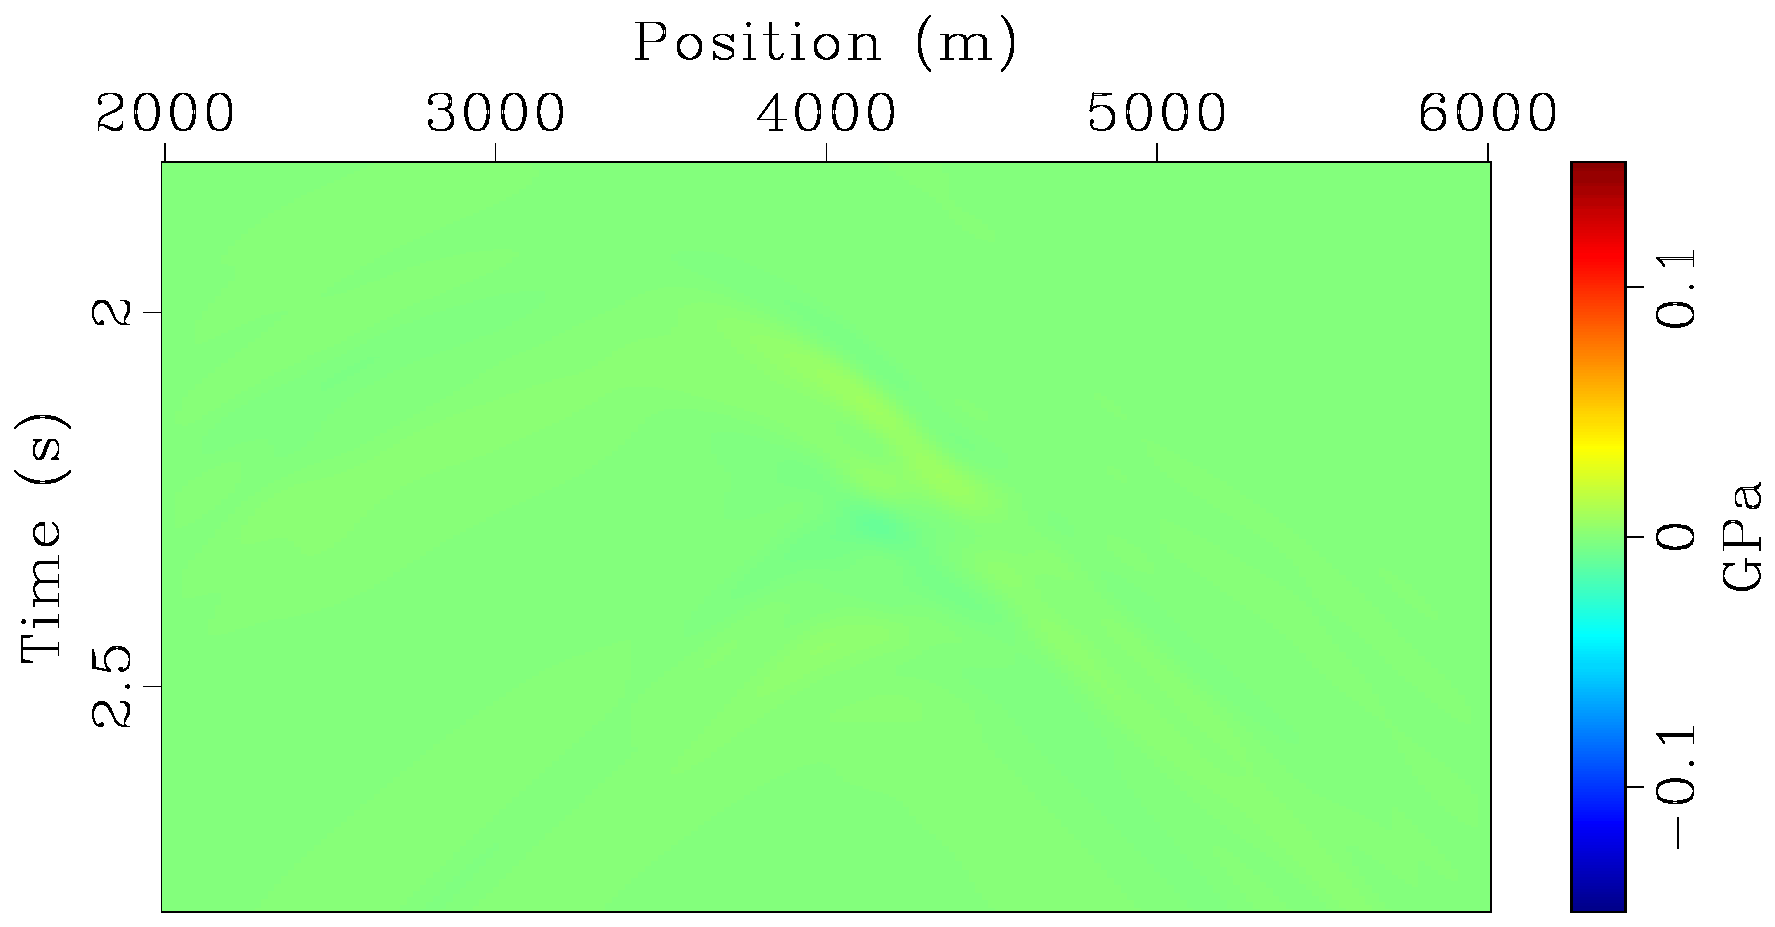
\includegraphics[height=1.25in]{Fig/residcovmestfwicgw41wind.pdf}\\
\vspace{0.25in}
Left: ``Jump to $\alpha=\infty$": bulk modulus estimated by FWI, 200
steepest descent steps starting with iteration 41 of SSE., final RMS residual reduction = 0.05;
Right: FWI data residual 
\end{center}
\end{frame}

\begin{frame}
  Why it works - a hint:

provided that
\begin{itemize}
\item $d = F[m_*]s$,
\item RMS wavelength of $w$ (hence $d$) $\rightarrow 0$,
\end{itemize}
\[
  \nabla \nabla  J_{\rm SSE}[m_*] \rightarrow \sum_{\bx,\bp}
\]
\end{frame}

\end{document}


\begin{frame}
\begin{center}
\vspace{-0.7in}
\includegraphics[height=4.5in]{HMC1.pdf}
\end{center}
\end{frame}

\begin{frame}
HMC Salt/Carbonate Acoustic Model

Streamer acquisition $z_s = 7$ m, $\Delta x_s=37.5$ m, 315 shots, $z_r=15$ m, $\Delta x_r=12.5$ m, 475 recvs, max offset = $6$ km

Pulse for data generation = [2, 3, 6, 10] Hz trapezoidal bandpass filter

Free surface @ $z=0$, other boundaries absorbing, 2-8 staggered FD scheme

Regularization: penalize MS velocity gradient, weight (also $\alpha$) via several trials

Data contains diving waves, pre- \& post-critical reflections, multiple reflections, refracted multiple reflections, head waves, free surface multiples, .... 

\end{frame}

\begin{frame}
\begin{center}
\vspace{-0.7in}
\includegraphics[height=4.5in]{HMC2.pdf}
\end{center}
\end{frame}

\begin{frame}
\begin{center}
\vspace{-0.7in}
\includegraphics[height=4.5in]{HMC3.pdf}
\end{center}
\end{frame}

\begin{frame}
\begin{center}
\vspace{-0.7in}
\includegraphics[height=4.5in]{HMC4.pdf}
\end{center}
\end{frame}

\section{Theory: why \& when it works}

\begin{frame}
FWI vs. SSE for transmission (diving wave, crosswell) data:

$J_{\rm FWI}[m]$ and $J_{\rm SSE}[m]$ = regular functions of $m$, locally close to quadratic approximations.

$d$ consistent: $d=Ru[m,f]$, $\of = f = w(t)\delta(\bx-\bx_s)$, $A\of=0$ $\Rightarrow$

\begin{itemize}
\item  $J_{\rm FWI}[m]=J_{\rm SSE}[m]=0$
\vspace{0.5cm}
\item $J_{\rm FWI}[m + \delta m] \approx \mbox{const. }\omega^2 \|\delta m\|^2$ for some $\delta m$ (kinematic perturbations), $\omega$ = center frequency in source pulse $w(t)$
\vspace{0.5cm}
\item $J_{\rm SSE}[m+\delta m] \le \mbox{const. }\|\delta m\|^2$ independent of $\omega, \delta m$
\end{itemize}
\end{frame}

\begin{frame}
$\Rightarrow$ radius of convexity region:
\begin{itemize}
\item $J_{\rm FWI}: O(1/\omega)$, must initialize ``within a wavelength''
\item $J_{\rm SSE}: O(1)$, converges even with (rel.) poor initial guess, HF data
\end{itemize}

Method of proof: ray theory (``mocrolocal analysis'')

More detailed analysis: minimizing $J_{\rm SSE}$ equivalent to a form of transmission travel time tomography: {\color{blue} tomography without picking} 

NB: for reflection data... ???
\end{frame}

\begin{frame}\frametitle{Late Breaking News}
Theory for special reflection case: layered ($\kappa(z)$) medium, dip filter to eliminate postcritical/diving wave energy

Explicit computation of $\nabla J_{\rm SSE}$ for 
\begin{itemize}
\item homogenous background 
\item data from single reflector in otherwise slowly varying $\kappa$, wavelet with central frequency $\omega$
\end{itemize}
$\Rightarrow$ $\nabla J_{\rm SSE} \rightarrow 0$ as $\omega \rightarrow \infty$

Same behavior as $\nabla J_{\rm FWI}$!!!

Upshot: for pure reflection data, SSE may not provide constructive velocity updates
\end{frame}

\begin{frame}
{\color{blue} {\bf Summary:}} Surface Source Extension 

\begin{itemize}
\item overcomes cycle-skipping for transmission data, solid theoretical foundation
\item same computational complexity as FWI
\item open question: theory for reflections {\color{blue} (initial result not positive)}
\end{itemize}
%\end{frame}

%\begin{frame}
Other source extension methods (WRI, AWI, ...)

\begin{itemize}
\item Many promising examples 
\item Little known theoretically - connection to travel time tomography???
\end{itemize}
\end{frame}

\begin{frame}\frametitle{Model Extension}
Add degrees of freedom to $v$, $\kappa$, instead of source

Annihilator: flatten/focus gathers

{\color{blue}Extracts velocity updates from reflection and refraction events} (S. 86, Kern \& S. 94, S. GP 08, Shen \& S. GEO 08, Shen EAGE 12, Biondi \& Almomin 12, 14, Chauris \& Cocher GEO 17, Hou \& S. GEO 18, Barnier \& Biondi SEG 19)

Chief challenge: expense(model extension) $\gg$ expense(FWI) (Note: expense(source extension) $\approx$ expense(FWI))
\end{frame}


\begin{frame}\frametitle{Acknowledgements}
\begin{itemize}
\item Total E\&P USA
\item Sponsors of The Rice Inversion Project
\item Organizers of SS 1 (Recent Advances and Road Ahead) at SEG 2019
\end{itemize}
\end{frame}

\end{document} 

\begin{frame}
Matched Source Waveform Inversion (Hua \& Symes 1993, 4, Huang \& Symes 2017) 

\begin{itemize}
\item similar to AWI (source wavelet for each trace), w/o normalization
\item if
\begin{itemize}
\item transmission data (crosswell, diving wave)
\item unique ray paths
\end{itemize}
then mean square moment $\approx$ mean square travel time misfit: {\color{blue} tomography without picking} 

\item relation with tomography fails ($\approx$ FWI) if multiple rays connect sources and receivers - contrast SSE
\end{itemize}
\end{frame}

\begin{frame}
\begin{center}
Example 2: Deep Water Marmousi
\end{center}
\begin{center}
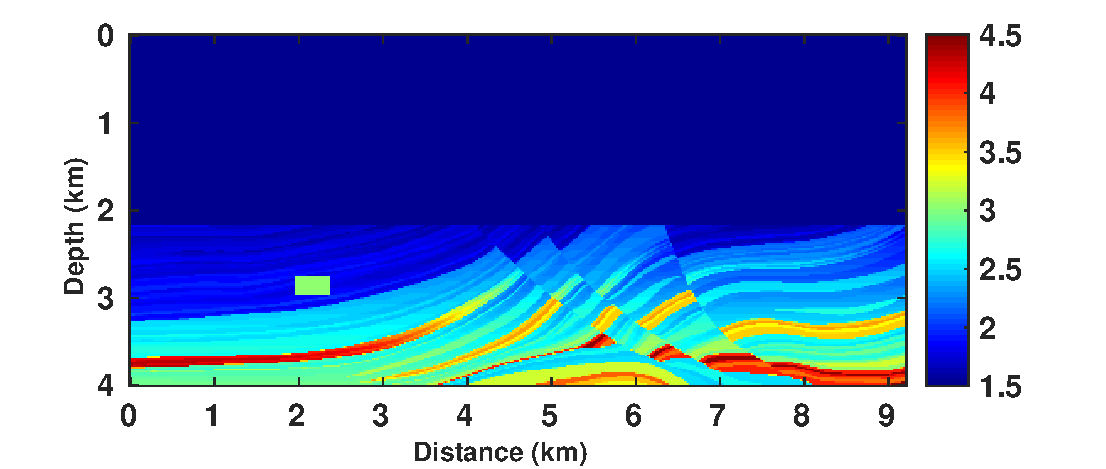
\includegraphics[height=2in,width=4in]{Fig/marm2km/Marm2kmVt.pdf}\\
Modified Marmousi Model: 2 km water layer added to minimize non-reflected energy, also box-snaped target
\end{center}
\end{frame}

\begin{frame}
\begin{center}
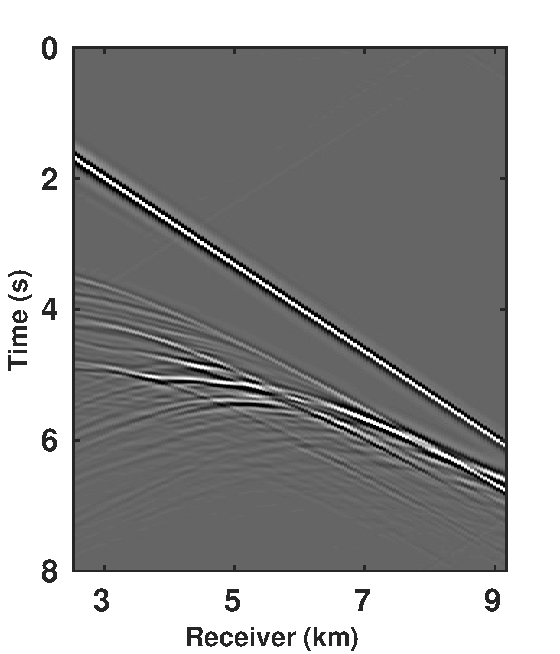
\includegraphics[height=2in]{Fig/marm2km/Marm2kmShot1}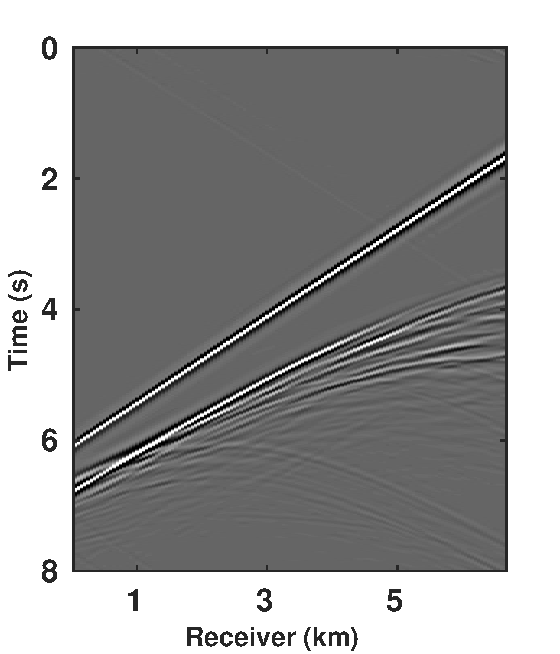
\includegraphics[height=2in]{Fig/marm2km/Marm2kmShot81}\\
Data: isotropic point source with 8 Hz Ricker wavelet, $z_r=0.04$ km, $x_r=$ 0.05 km to 9.15 km, $\Delta x_r=$ 0.05 km, $z_s=0.08$ km, $x_s=0.6$ km to $x_s=8.6$, $\Delta x_s$ = 0.1 km. Shots at $x_s=0.6$ km and $x_s=8.6$ km displayed.
\end{center}
\end{frame}

\begin{frame}
\begin{center}
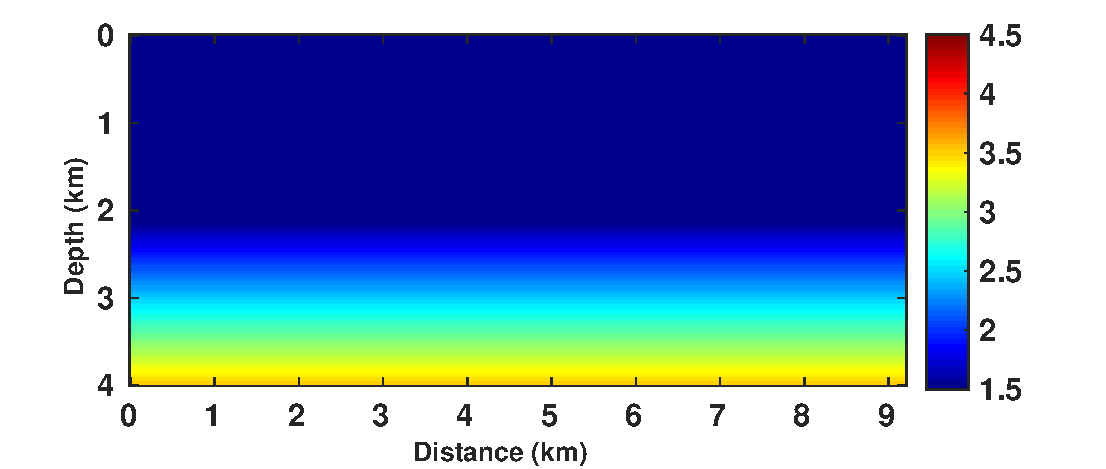
\includegraphics[height=2in,width=4in]{Fig/marm2km/Marm2kmV0.pdf}\\
Initial $v(z)$ model for both FWI and SSE
\end{center}
\end{frame}

\begin{frame}
\vspace{-0.1cm}
\begin{center}
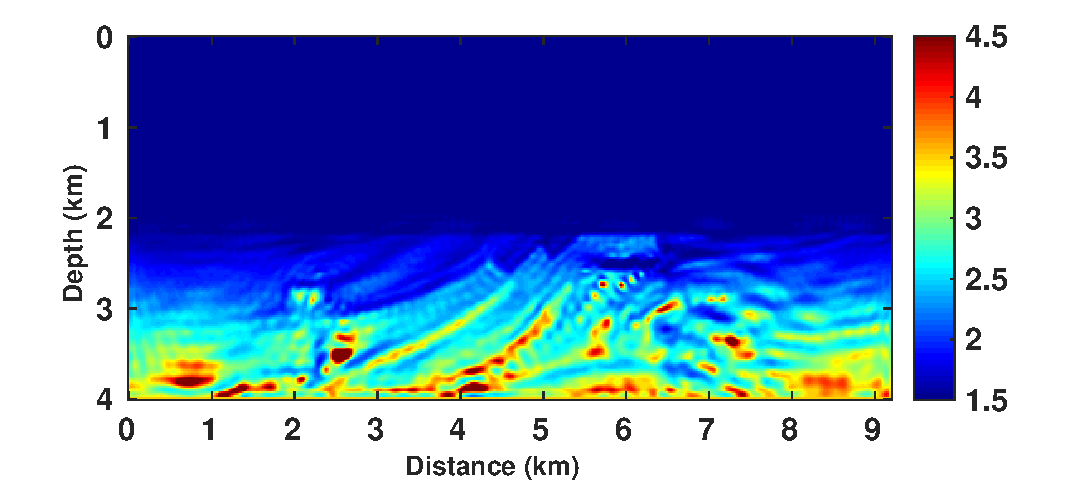
\includegraphics[height=2in,width=4in]{Fig/marm2km/Marm2kmFWI.pdf}\\
FWI estimate of $v$: 200 iterations LBFGS, frequency domain FD 5-8 Hz
\end{center}
\end{frame}

\begin{frame}
\begin{center}
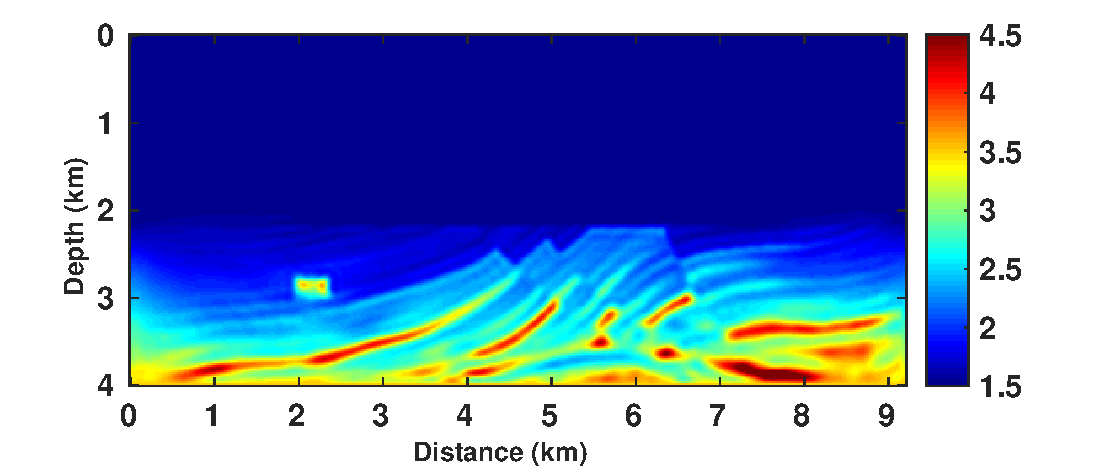
\includegraphics[height=2in,width=4in]{Fig/marm2km/Marm2kmSurf.pdf}\\
SSE estimate of $v$: 150 iterations LBFGS, frequency domain FD 5-8 Hz, fixed $\alpha$ set by trial
\end{center}
\end{frame}

\begin{frame}
%\vspace{0.07cm}
\begin{center}
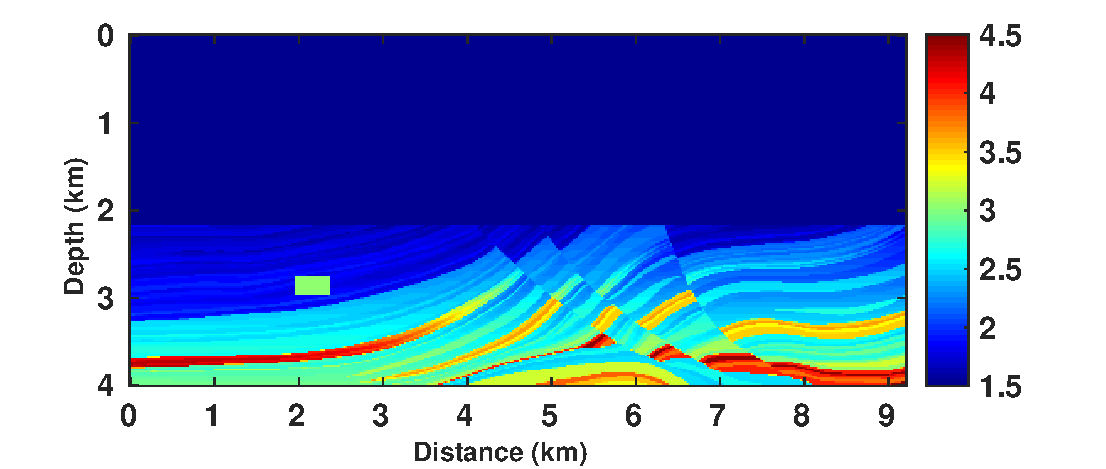
\includegraphics[height=2in,width=4in]{Fig/marm2km/Marm2kmVt.pdf}\\
Modified Marmousi Model: 2 km water layer added to minimize non-reflected energy, also box-snaped target
\end{center}
\end{frame}

\begin{frame}
\begin{center}
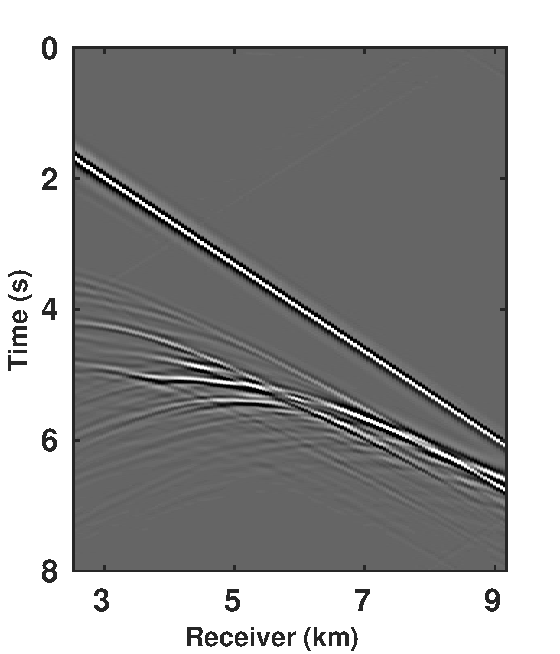
\includegraphics[height=2in]{Fig/marm2km/Marm2kmShot1Inv}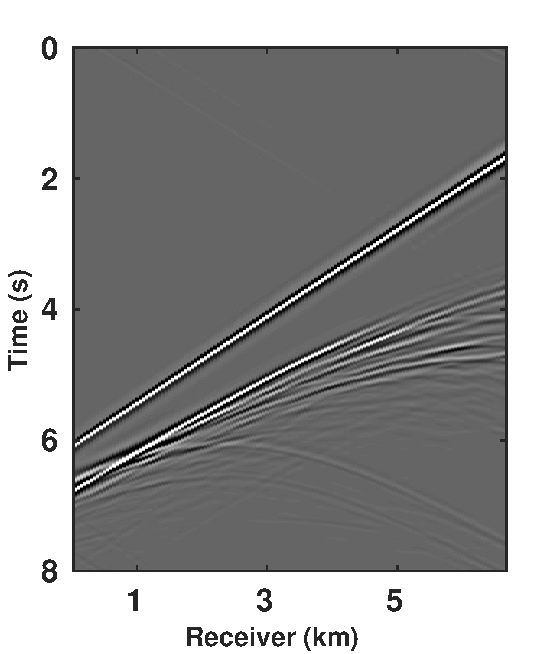
\includegraphics[height=2in]{Fig/marm2km/Marm2kmShot81Inv}\\
Data predicted from SSE inverted model: shots at $x_s=0.6$ km and $x_s=8.6$ km.
\end{center}
\end{frame}

\begin{frame}
\begin{center}
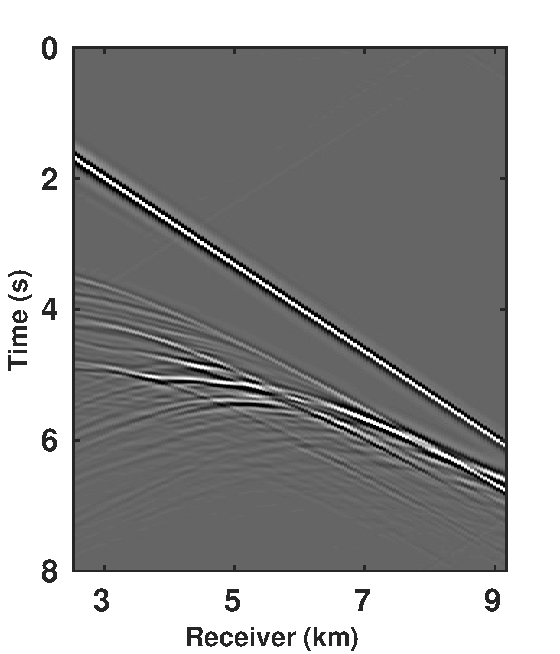
\includegraphics[height=2in]{Fig/marm2km/Marm2kmShot1}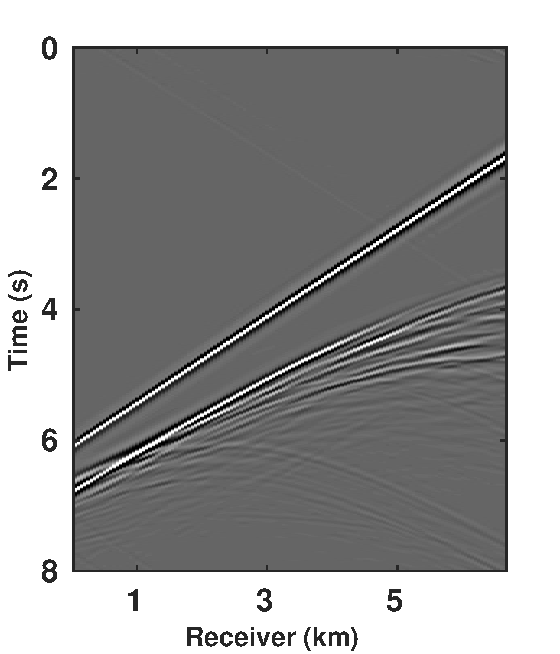
\includegraphics[height=2in]{Fig/marm2km/Marm2kmShot81}\\
Target data:\\ shots at $x_s=0.6$ km and $x_s=8.6$ km.
\end{center}
\end{frame}

\begin{frame}
Wavefield Reconstruction Inversion: $\of(\bx,t;\bx_s)$ distributed throughout space-time

van Leeuwen and Herrmann 2013, 2016, Wang \& Yingst 2016 

similar: space-time extension Huang \& S. 2018 

\begin{itemize}
\item[+ ]many good examples, convincing numerical evidence
\item[+ ]3D field data - Wang \& Yingst 2016
\item[- ]basic form: store complete space-time (or space-frequency) fields (6D)
\end{itemize}
\end{frame}

\begin{frame}
Adaptive Waveform Inversion (Warner \& Guatsch, 2014, 2016): $\of(\bx,t;\bx_r,\bx_s) = w(t;\bx_r)\delta(\bx-\bx_s)$ localized but depends on receiver coordinate $\bx_r$ - one wavelet per data trace

similar: source-receiver extension Hua \& S. 1994, Huang \& S. 2017

\begin{itemize}
\item[+ ]additional storage: $\approx$ data volume (5D)
\item[+ ]minor mod of standard FWI workflow
\item[- ]source-receiver: loses advantage over FWI when sources, receivers connected by multiple ray paths (fails for lens model, above)
\end{itemize}
\end{frame}

\begin{frame}
Intermediate: source distributed over space-time surface
\begin{itemize}
\item const. t surface = volume source extension - Huang \& S. 2018
\item const z surface = {\color{blue} surface source extension (SSE):} 
\[
\of(\bx,t;x_s,y_s) = w(x,y; x_s,y_s)\delta(z-z_s)
\]
\end{itemize}
\begin{itemize}
\item[+ ]additional storage = O(data volume) (5D)
\item[+ ]no problem with multiple ray paths
\item[+ ]theory for transmission data (eg. diving wave): {\color{blue} tomography w/o picking}
\end{itemize} 
\end{frame}

